\chapter{Results}
Using a simulated environment we evaluate how application performance is impacted when using a network of primary memory devices, where latency will inherently increase with each hop. In this chapter we will go through each application's access time pattern and behaviour by first measuring using one single HMC device, with a single link hop. Then we will increase the number of devices and always use the device at the end of the chain, e.g. when having seven devices we will perform all allocations on the seventh device. At the same time, we will run each configuration with both two and four links. We will view these results both from a device and an application perspective. Finally, we present a summary of our findings.


\section{MCF}
The first application to be run is the, arguably, most memory intensive and latency sensitive benchmark in the SPEC2006 suite - 429.mcf. Figure \ref{Memory-access-429-single}, visualising access times when a single HMC device is being used, shows that there is a large variance in latency during application run time, even though the only contention available is from its own memory requests. Additionally, there are notable peaks present at precisely 93 ns intervals. In-between the aforementioned peaks the pattern looks quite similar with the differences mostly accredited to resolution in terms of occurrences of requests with specific latency.
\bigskip

\begin{figure}[!ht]
    \centering
    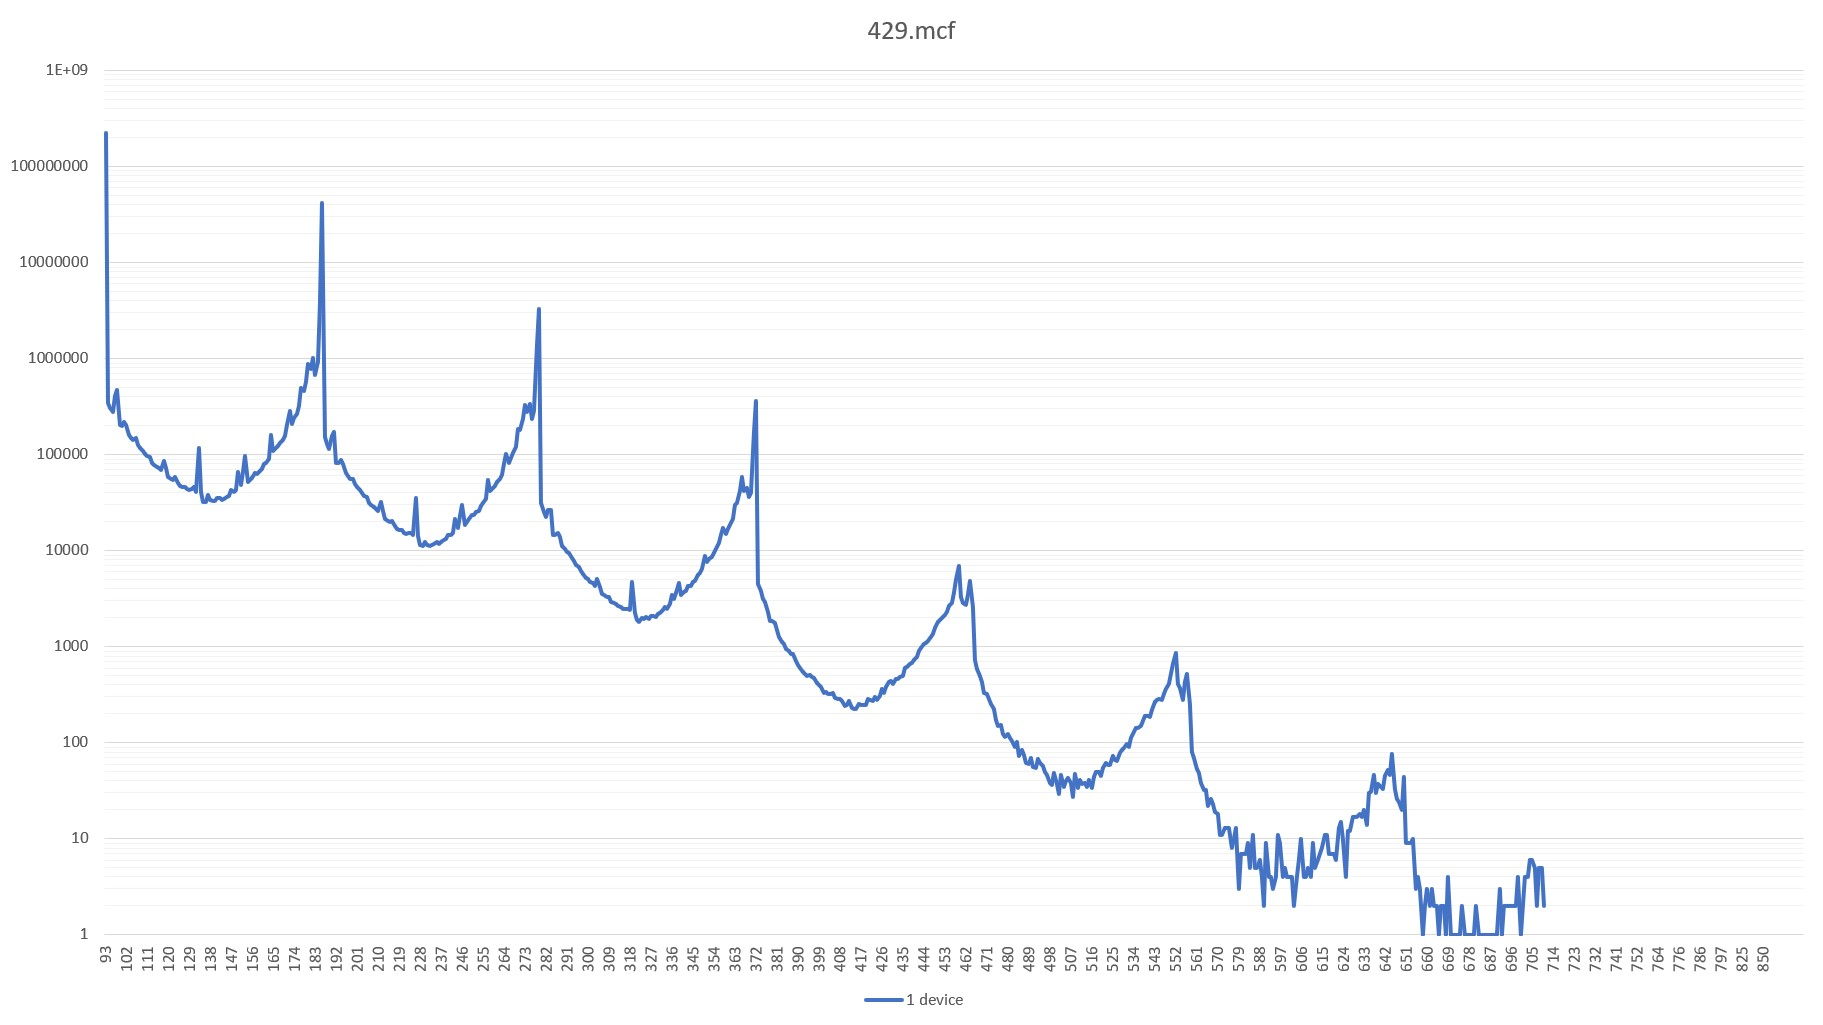
\includegraphics[width=1.0\linewidth]{figure/429-x_4-1.jpg}
    \caption{Access times using one device with two links, running 429.mcf.}
    \label{Memory-access-429-single}
\end{figure}

The reason there are peaks at 93 ns interval is because the queues fill up faster than data can be fetched from banks. An application with a high number of memory requests will increase the memory system's overall request latency \cite{8366939}. Latency for a request is dependent on both how quickly data can be retrieved plus the time taken to serve all other requests ahead in the queue. With just one application running, there will only be requests thence to take into account. Moreover, applications issue large amounts of consecutive memory requests when streaming data from memory. While mcf has some streaming behaviour it is less than 30\% of the time, though it tends to request large datasets at a time \cite{10.1145/3307650.3322229}. This is enough to create congestion in the queues and resulting in request latency being multiples of 93 ns, which is the latency set for DRAM lookup.
\bigskip

Adding more devices, and thereby placing data further from the host, will incur greater latencies as seen in figure \ref{Memory-access-429}. However, it can be noted that the peaks all have about the same magnitude and the repeating pattern in between is reminiscent of each other but with a few differences. These variations should be due to contention arising on the links when data to and from far-away devices tries to use the same links. While the links themselves are duplex and allows traffic in both directions simultaneously, the queues can get full if enough data is pushed in a small time frame. This means that contention exists, but should stay virtually unchanged over multiple network hops while running a single application. Furthermore, comparing the access time patterns of using one device and three, in figure \ref{Memory-access-429-double}, we can see that there are differences in latency distribution, but the main peaks at 93 ns interval remain the same. In addition, disregarding the initial latency we also calculate that the average latency is the same at 117 ns.
\bigskip

\begin{figure}[!ht]
    \centering
    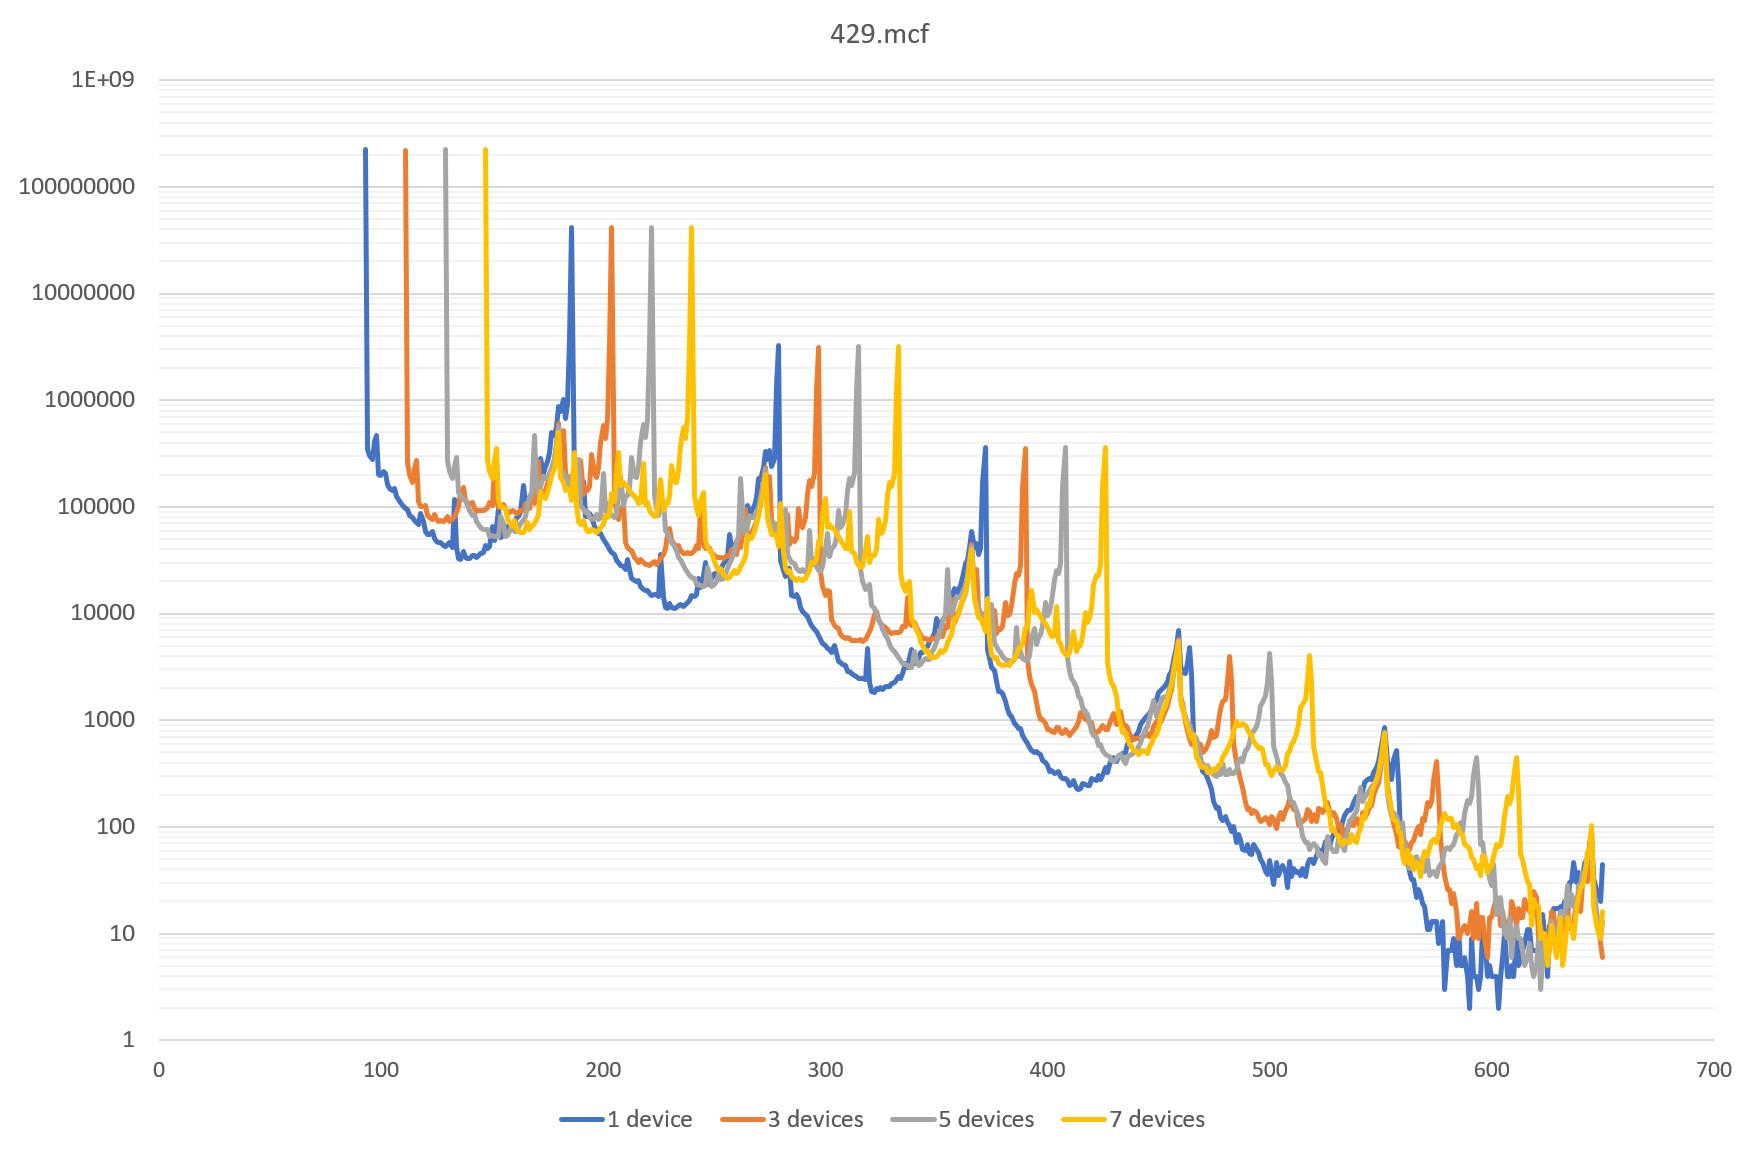
\includegraphics[width=1.0\linewidth]{figure/429-x_4.jpg}
    \caption{Comparing access times when using one, three, five and seven devices.}
    \label{Memory-access-429}
\end{figure}

\begin{figure}[!ht]
    \centering
    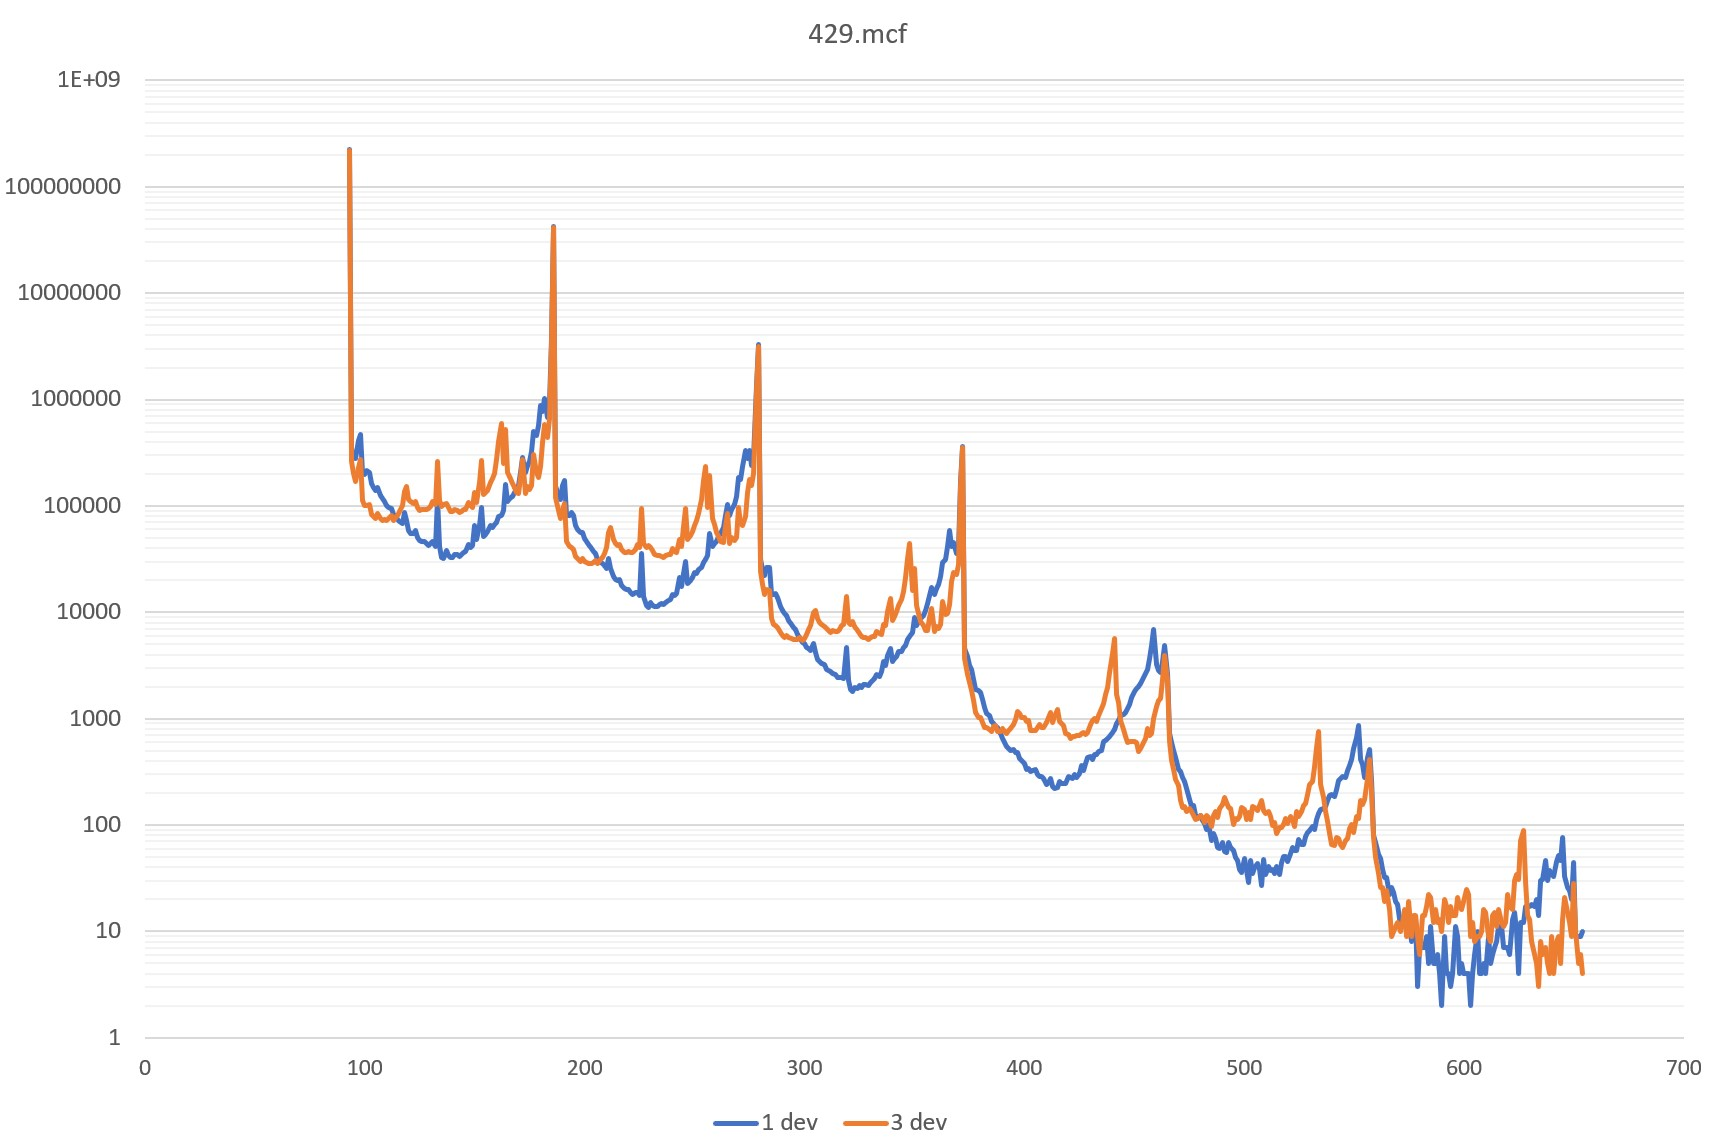
\includegraphics[width=1.0\linewidth]{figure/429-x_4-2.jpg}
    \caption{Access time patterns for one and three devices, where the latter has been adjusted to compensate for initial latency.}
    \label{Memory-access-429-double}
\end{figure}

Next we run using more links between the host and first device, as well as between individual cubes. Specifically, we now simulate using four links instead of the previous two. This should to some extent alleviate the contention issue, but since the access scheme of the links is a simple round robin there might also be some added waiting time before data gets to the host. Running mcf using four active links and more than four devices turned out to take too long time (excess of two months run time) and those simulations were finally terminated.
\bigskip

\begin{figure}[!ht]
    \centering
    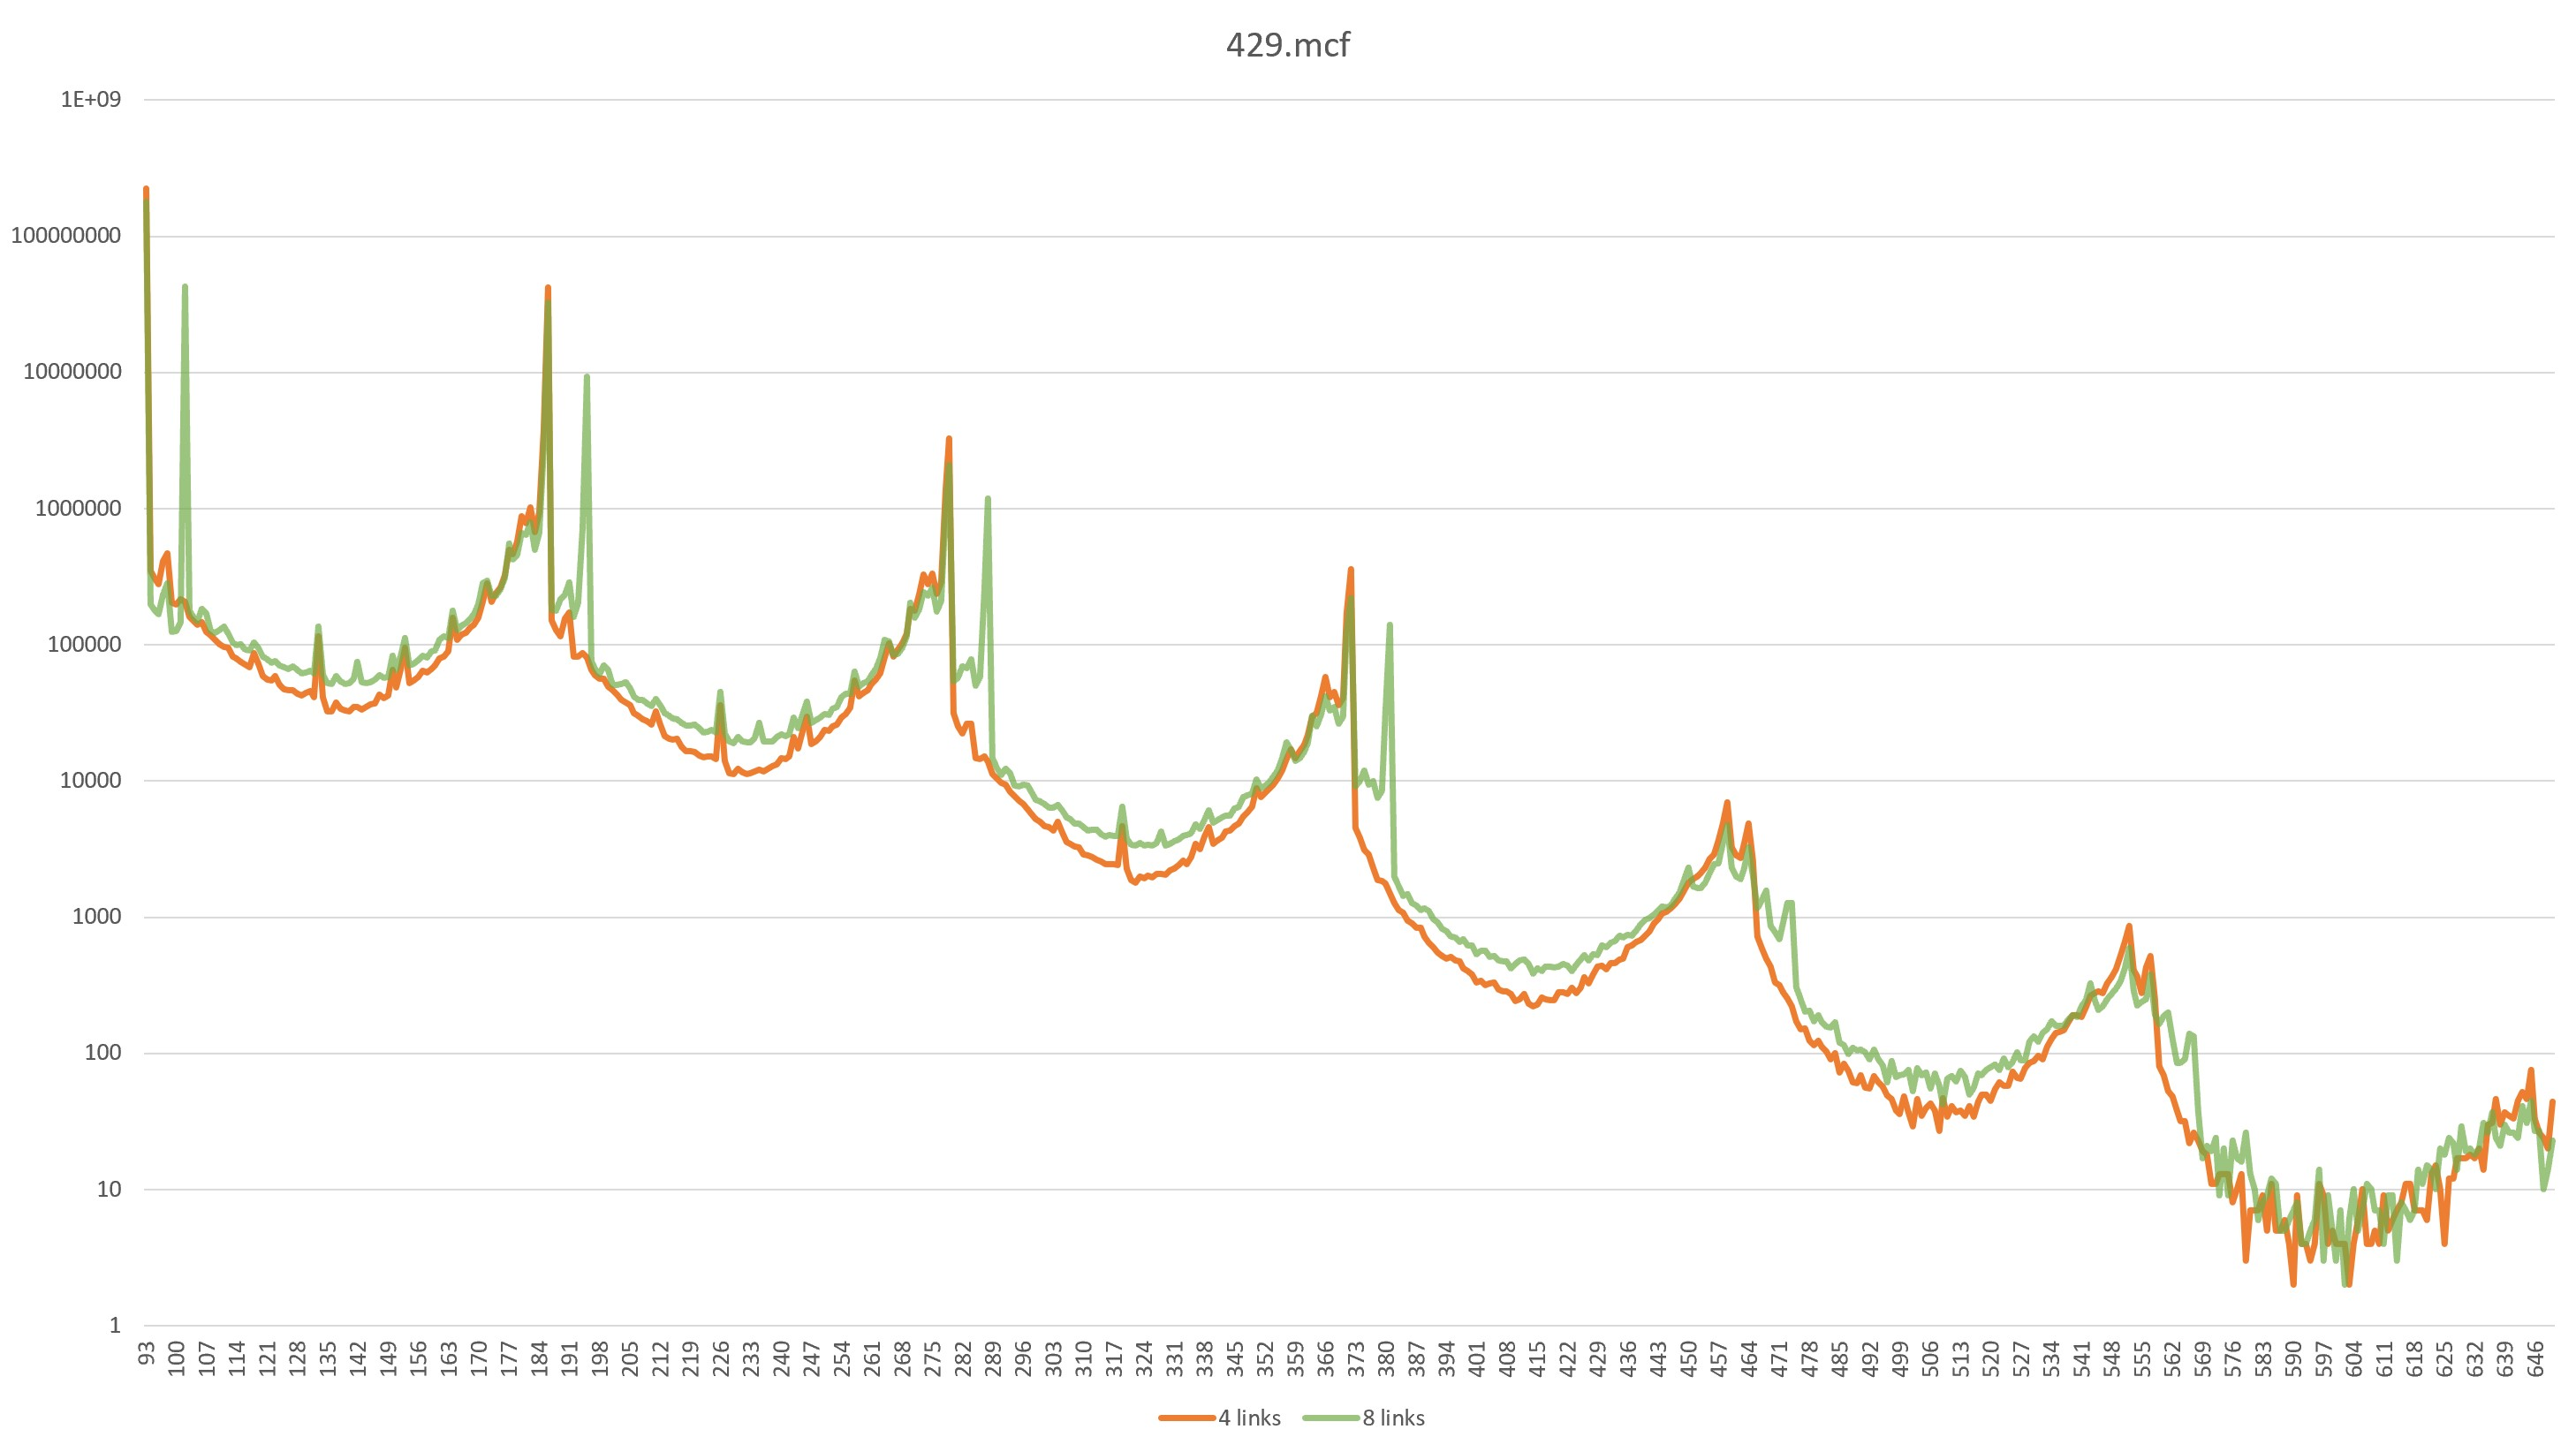
\includegraphics[width=1.0\linewidth]{figure/429-2_4-8.jpg}
    \caption{Part of the access patterns for one and two devices, where the latter has been adjusted to compensate for initial latency.}
    \label{Memory-access-429-link-compare}
\end{figure}

Running mcf using four links produces some unexpected results. As can be seen in figure \ref{Memory-access-429-link-compare} the access time pattern looks very similar to using only two links, but there are new trailing spikes at 9 ns after the bigger peaks. The second spike is a split of the otherwise always present peaks with 93 ns interval, where close to 20\% of those accesses are delayed with 9 ns. If data is sent down a link that is attached to another vault, there will have to be internal routing done by the logic layer which could delay the request. By increasing bandwidth, through increased parallelism, we potentially worsen performance for this single application. However, when using three cubes, i.e. adding a hop, the patterns look almost identical. As such, the added latency of multiple links is masked when having longer network traversal time. 
\bigskip

Average latency increases with added network hops, as can be expected, but it also increases somewhat when utilising more parallelism, as seen in figure \ref{Memory-access-429-average-latency}. Comparing average latencies when allocating data on different distances shows that latency increases with 18 ns for every additional hop. Observing figure \ref{Memory-access-429-exectime}, we can notice that execution time for mcf increases with higher average latency. It is hard to determine from looking at the figures how latency sensitivie mcf really is, but execution time increases at most by about 38\% while average latency tops out at 45\% higher.

\begin{figure}[!ht]
    \centering
    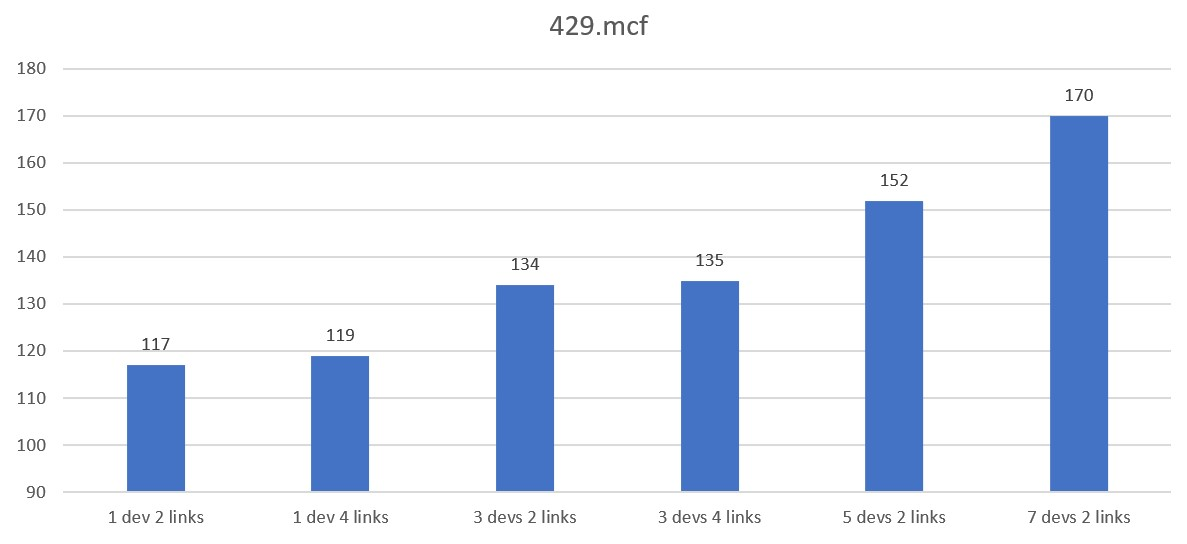
\includegraphics[width=1.0\linewidth]{figure/429-averages.jpg}
    \caption{Comparing average latency between configurations.}
    \label{Memory-access-429-average-latency}
\end{figure}

\begin{figure}[!ht]
    \centering
    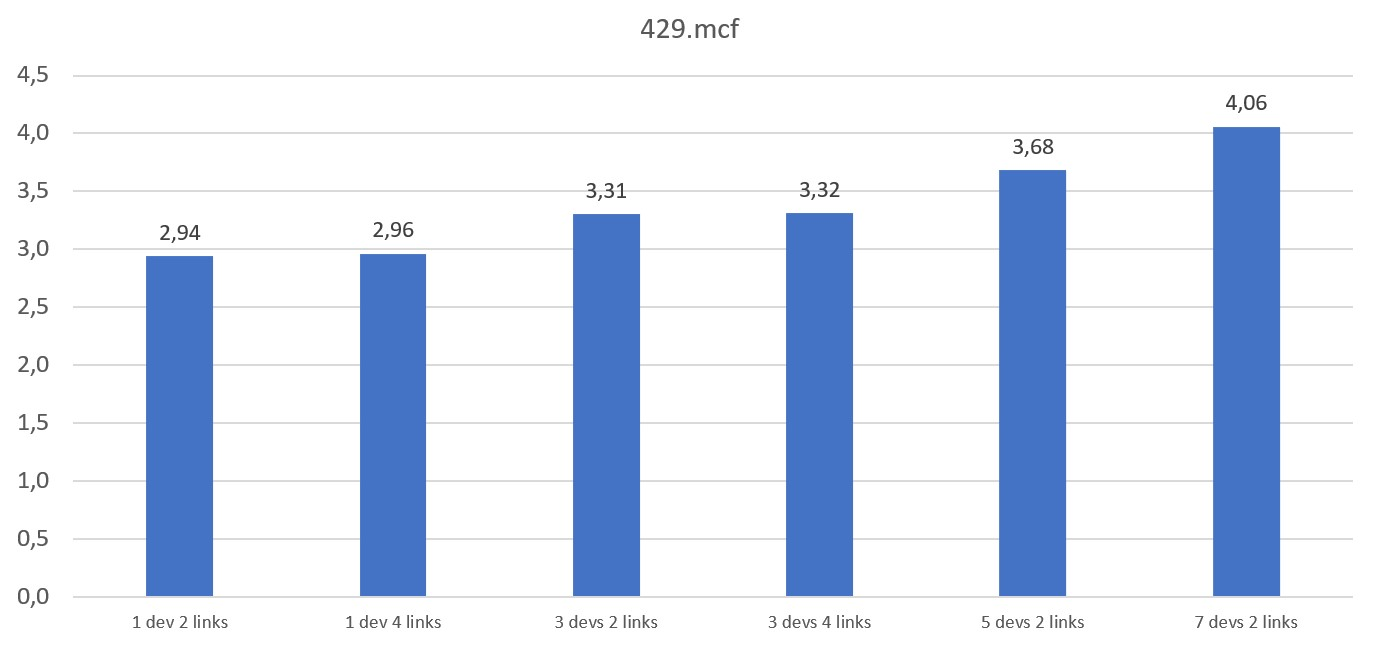
\includegraphics[width=1.0\linewidth]{figure/429-exectime.jpg}
    \caption{Execution time in seconds for different configurations.}
    \label{Memory-access-429-exectime}
\end{figure}

\section{NAMD}
444.namd is a mostly compute bound application. This should make access patterns look a little different based on how much data is accessed at a time. In figure \ref{Memory-access-444} we can see what those patterns look like using one, three, five and seven cubes in the network. While there is a pattern between 93 and 186 ns which look quite similar between the configurations, the number of memory requests are too low overall which quickly decreases the resolution and makes patterns almost indiscernible. Many requests do not return immediately, i.e. having a latency of 93 ns, but instead has a higher latency; the most requests are served after 186 ns, which is double that of the minimal possible latency. Namd performs a lot of array lookups and it could be this often-accessed array of subsequent elements we are seeing being used. %Additionally, it might be that the introduced MLP hurts performance because the gain of higher bandwidth is outweighed by the overhead of having to wait for internal routing inside the cube. Sadly HMCSim cannot be configured using one single link and thus there is no easy way to verify this claim here.
\bigskip

While mcf can utilise the memory quite well, although having noticeable congestion in queues, the average latency shows that a large enough portion of all accesses are performed in 93 ns. Conversely, it is clear from figure \ref{Memory-access-444} that namd behaves differently. More than 60\% of Namd's memory accesses are streams, effectively increasing strain on the queues and thereby increasing latency \cite{10.1145/3307650.3322229}. Furthermore, the memory stream accesses happens in bursts and appears to be intensive enough to cause most requests having to wait for 186 ns; despite the total number of requests being relatively few for namd, the burst-like access pattern negatively affects the average latency
\bigskip

\begin{figure}[!ht]
    \centering
    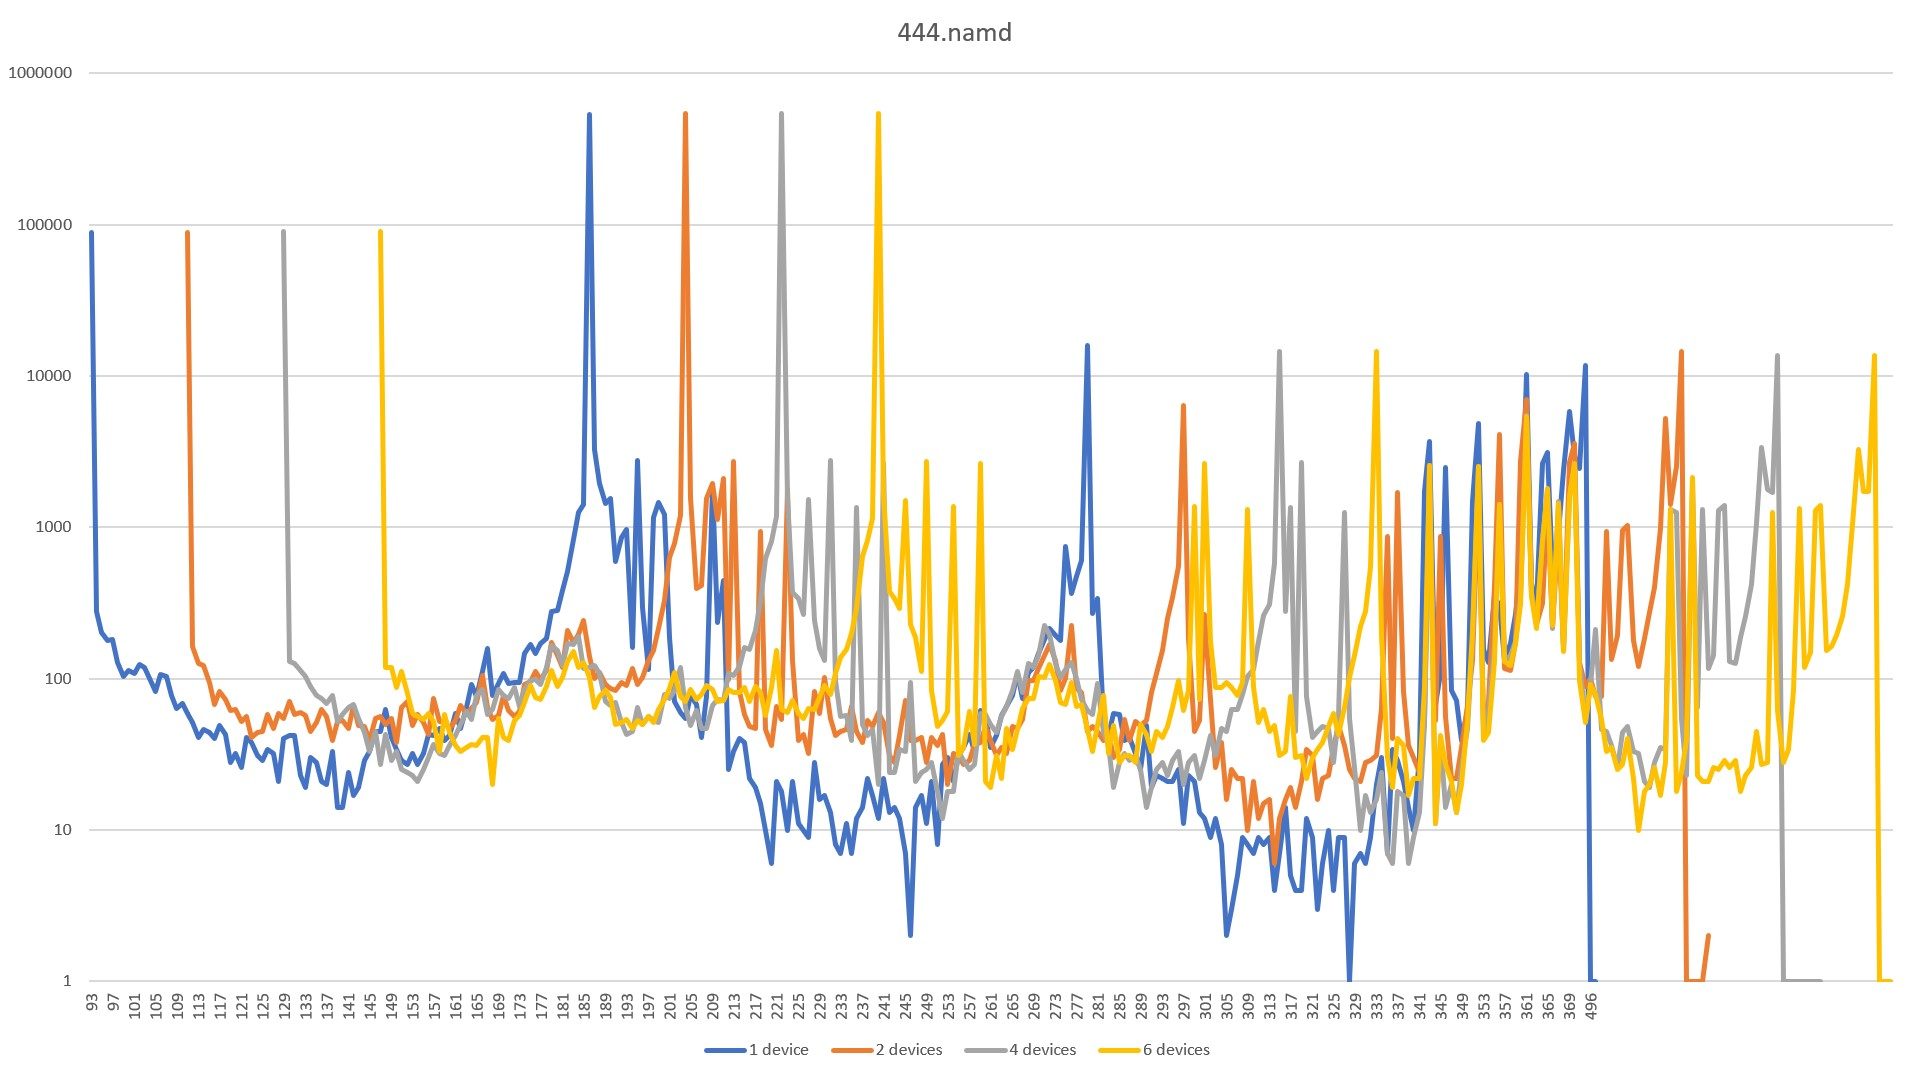
\includegraphics[width=1\linewidth]{figure/444-x_4-1.jpg}
    \caption{Comparing access times when using one, three, five and seven devices.}
    \label{Memory-access-444}
\end{figure}

Doubling the number of links, using four instead of two, will further hamper the application in terms of latency. Interestingly, the same behaviour as was seen in the mcf results are seen in figure \ref{Memory-access-444-links-compare} as well. There are new peaks added 9 ns after the otherwise normally present peaks. In addition, this spike has a much greater impact on this application's average latency compared to mcf, adding five ns as compared to two ns. Because the split spikes represents a larger portion of all memory accesses for namd, it affects the average a lot -- there are more accesses at 195 ns than at 93. In addition, the averages for namd are overall notably higher than those for mcf. Moreover, there are notably latency penalties seen even when using four links and allocating data on the seventh device. However, in the end, as can be seen in figure \ref{Memory-access-444-average-latency}, the biggest hit to performance is taken when introducing new hops. 
\bigskip

\begin{figure}[!ht]
    \centering
    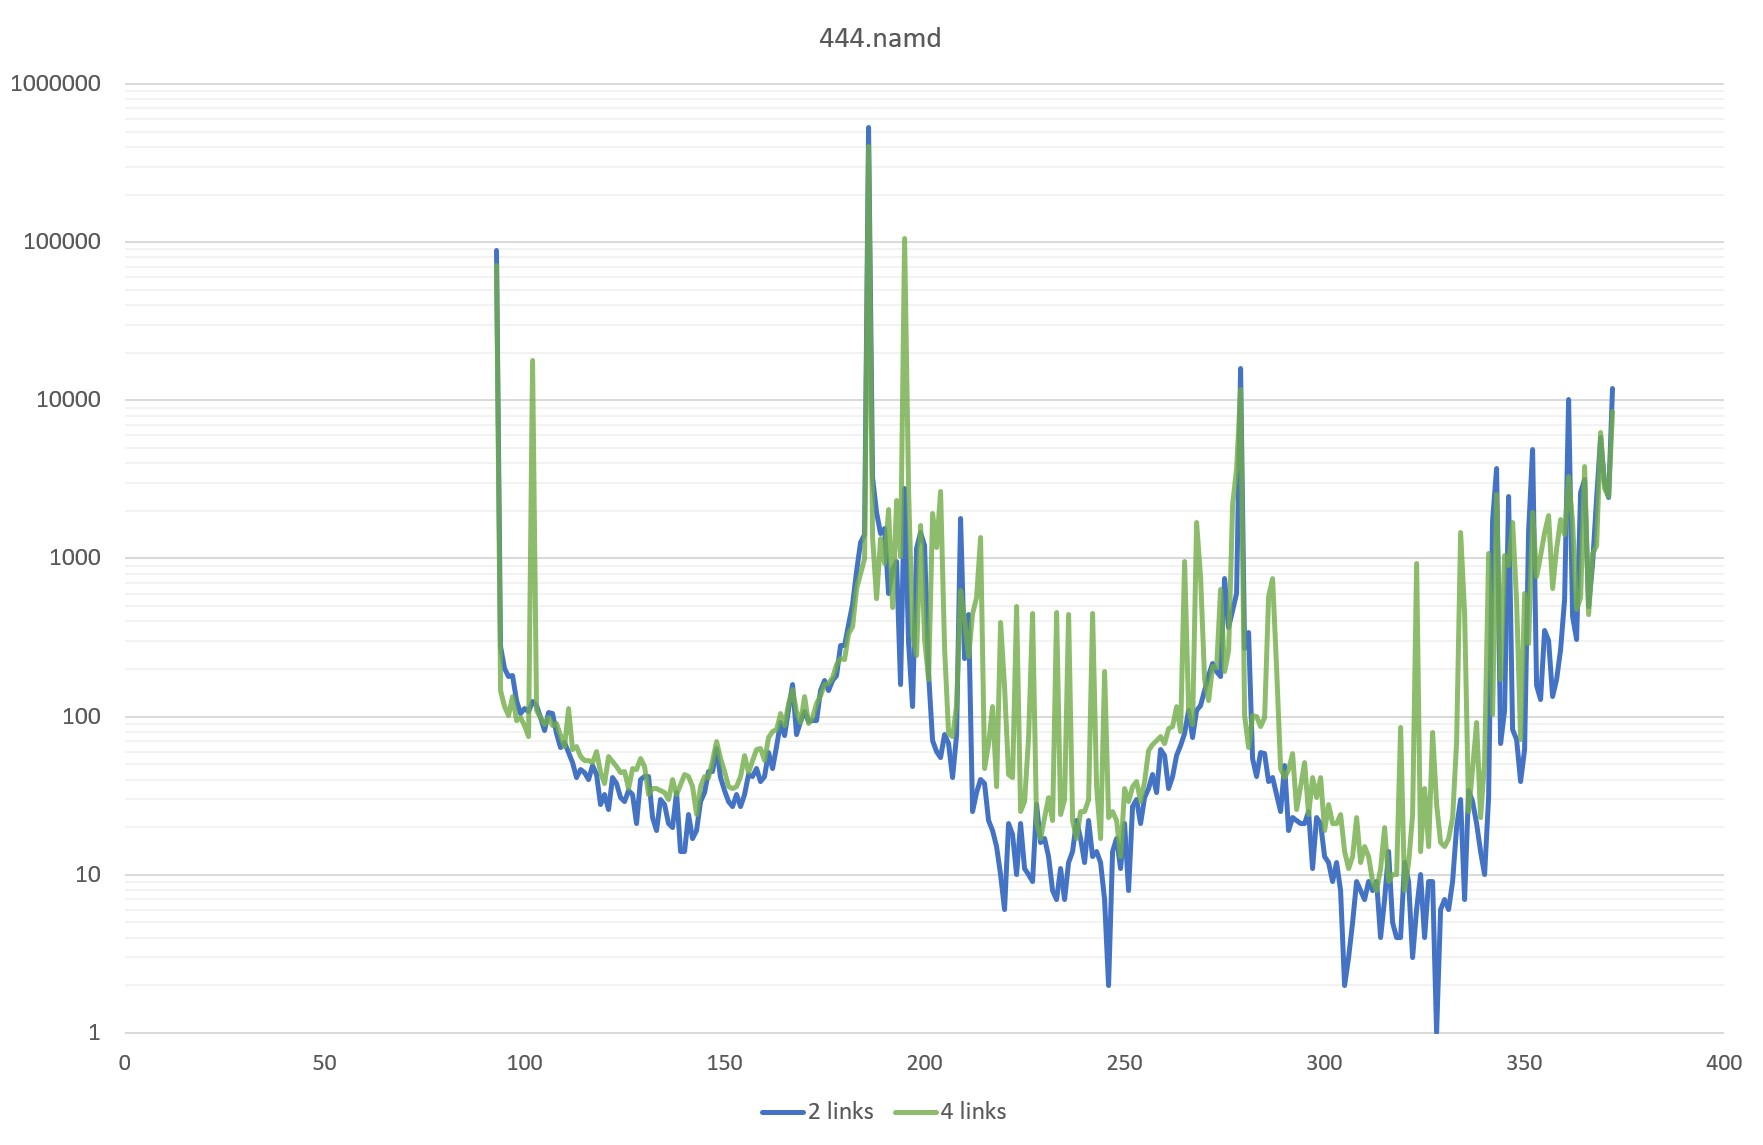
\includegraphics[width=1.0\linewidth]{figure/444-2_4-8.jpg}
    \caption{Comparing latencies when using two and four links using one single device.}
    \label{Memory-access-444-links-compare}
\end{figure}

\begin{figure}[!ht]
    \centering
    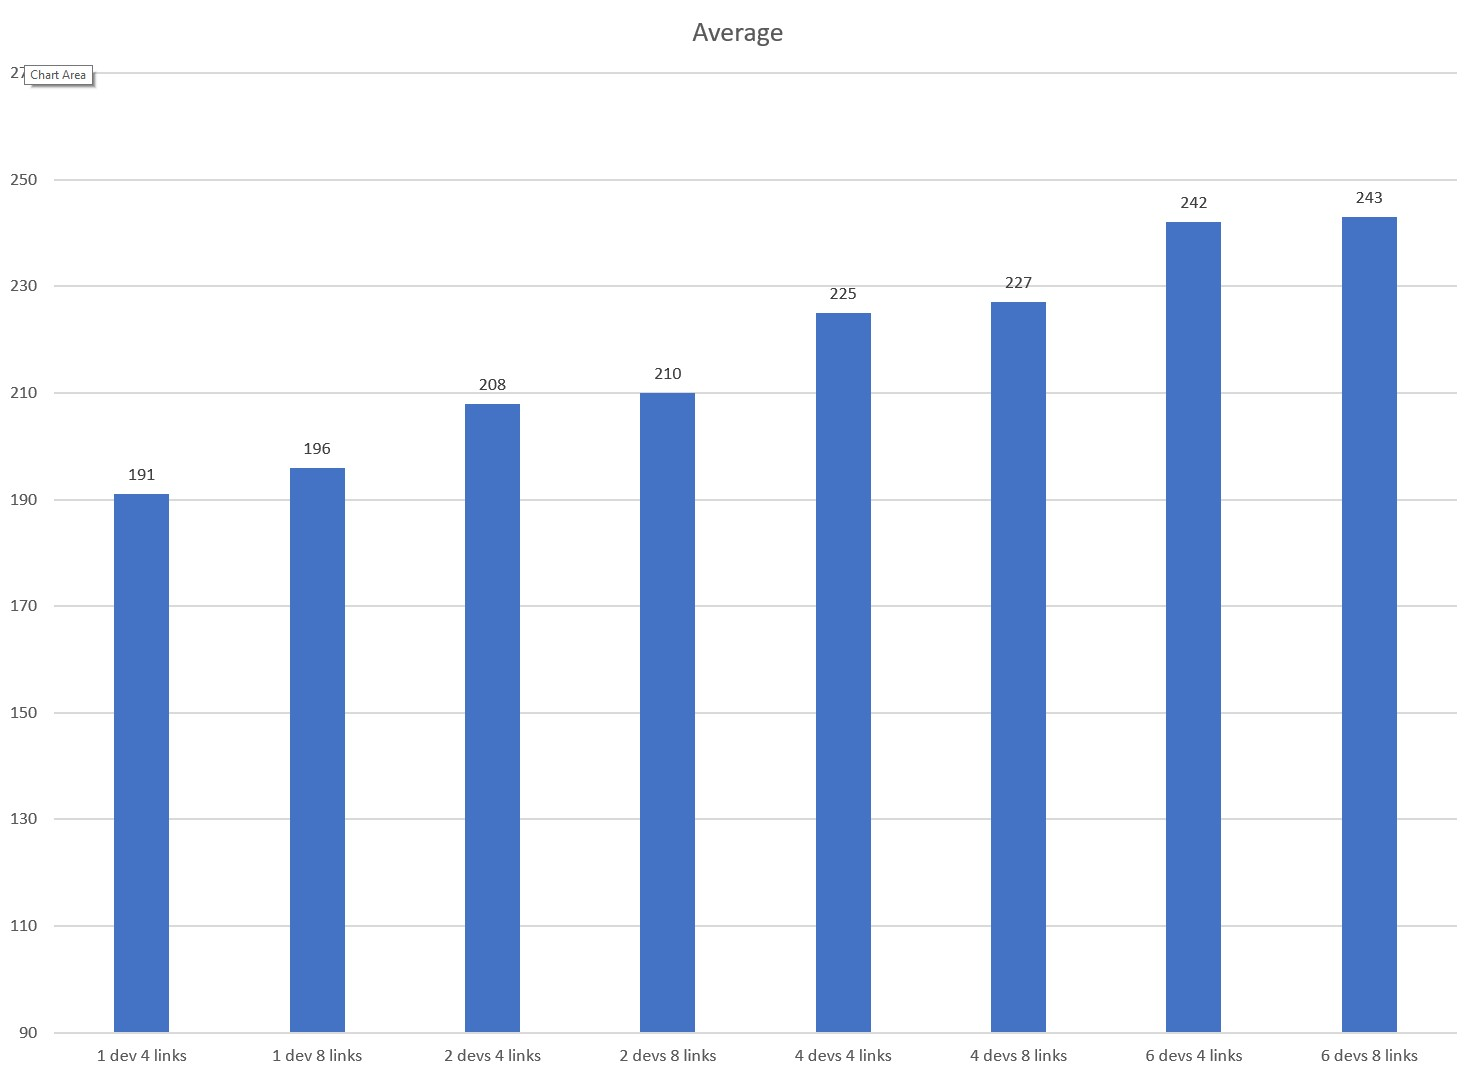
\includegraphics[width=1.0\linewidth]{figure/444_averages.jpg}
    \caption{Comparing average latency between configurations.}
    \label{Memory-access-444-average-latency}
\end{figure}

Namd is a compute bound application, and while its average latencies are comparably high, its performance is not affected very much. Figure \ref{Memory-access-444-exectime} shows that only an additional 12 ms is added to the total execution time in the worst case. 

\begin{figure}[!ht]
    \centering
    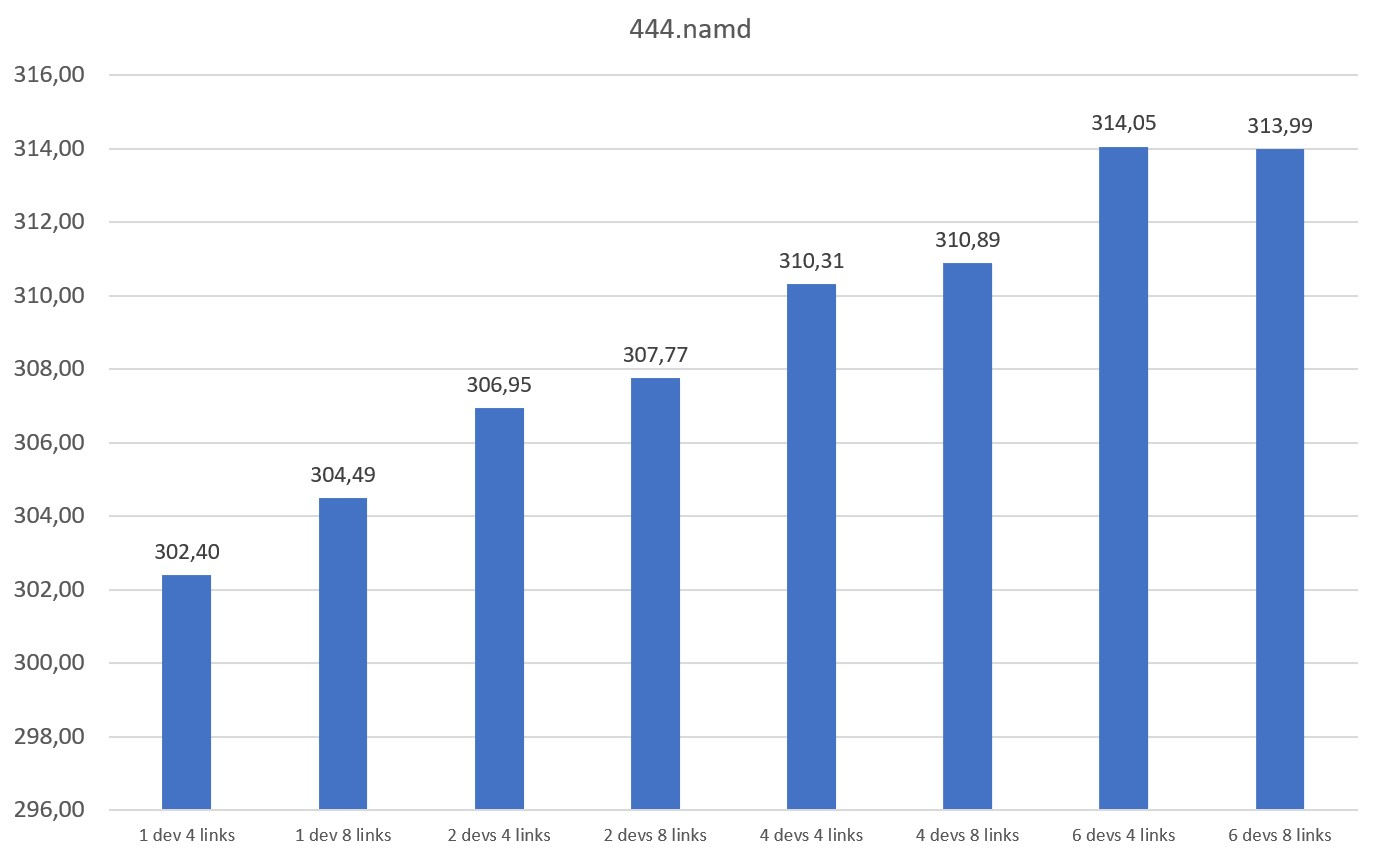
\includegraphics[width=1.0\linewidth]{figure/444-exectime.jpg}
    \caption{Execution time in ms for different configurations.}
    \label{Memory-access-444-exectime}
\end{figure}

\section{SOPLEX}
450.soplex is a linear program where every iteration depends on the last. As such, while the application is memory intensive, increased MLP is not expected to yield significant improvements for the general algorithm. However, when starting to look at the average latencies for the different configurations we notice an unexpected result, as seen in figure \ref{Memory-access-450-average-latency}. Having four devices with four links generates, marginally, better results with respect to the average latency. It is hard to determine what exactly made the difference, since, as can be seen in the comparative figure \ref{Memory-access-450-4-dev-4-8-links}, the access time patterns between using two and four links on the third device look more or less identical. In addition, the averages are rounded down -- the values could both have been close to 122 but rounded differently. In the end, this result could be interpreted as being within the margin of error and the real results be seen as more or less equal.
\bigskip

\begin{figure}[!ht]
    \centering
    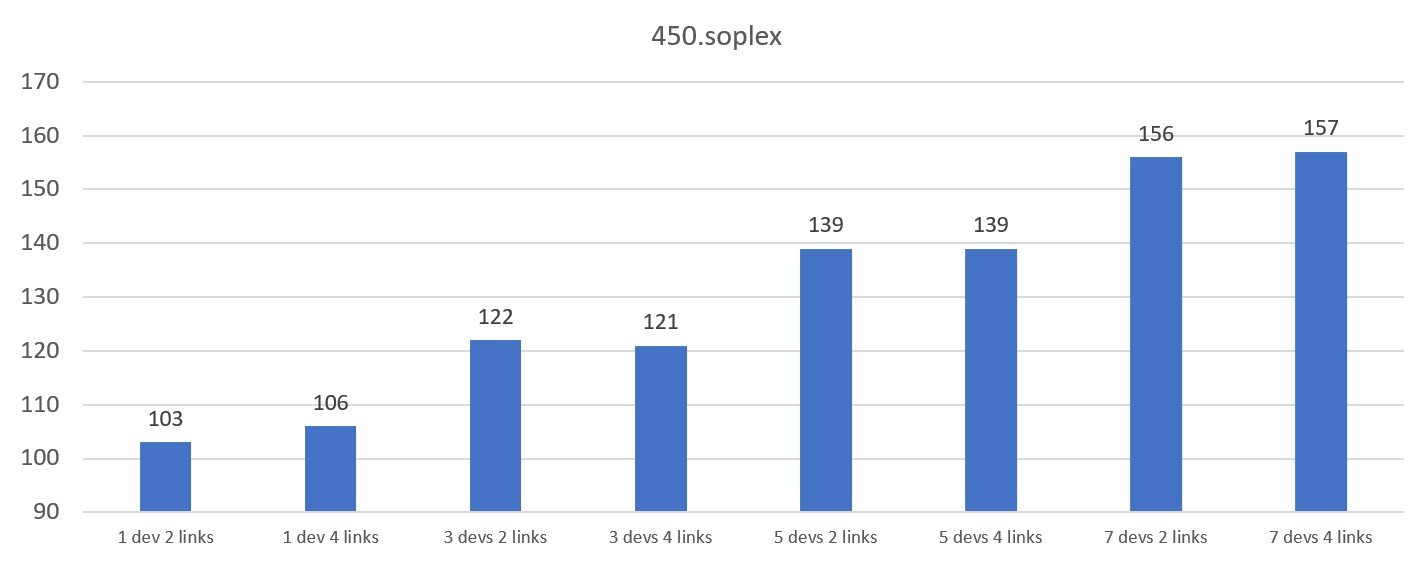
\includegraphics[width=1.0\linewidth]{figure/450-averages.jpg}
    \caption{Comparing average latency between configurations.}
    \label{Memory-access-450-average-latency}
\end{figure}

\begin{figure}[!ht]
    \centering
    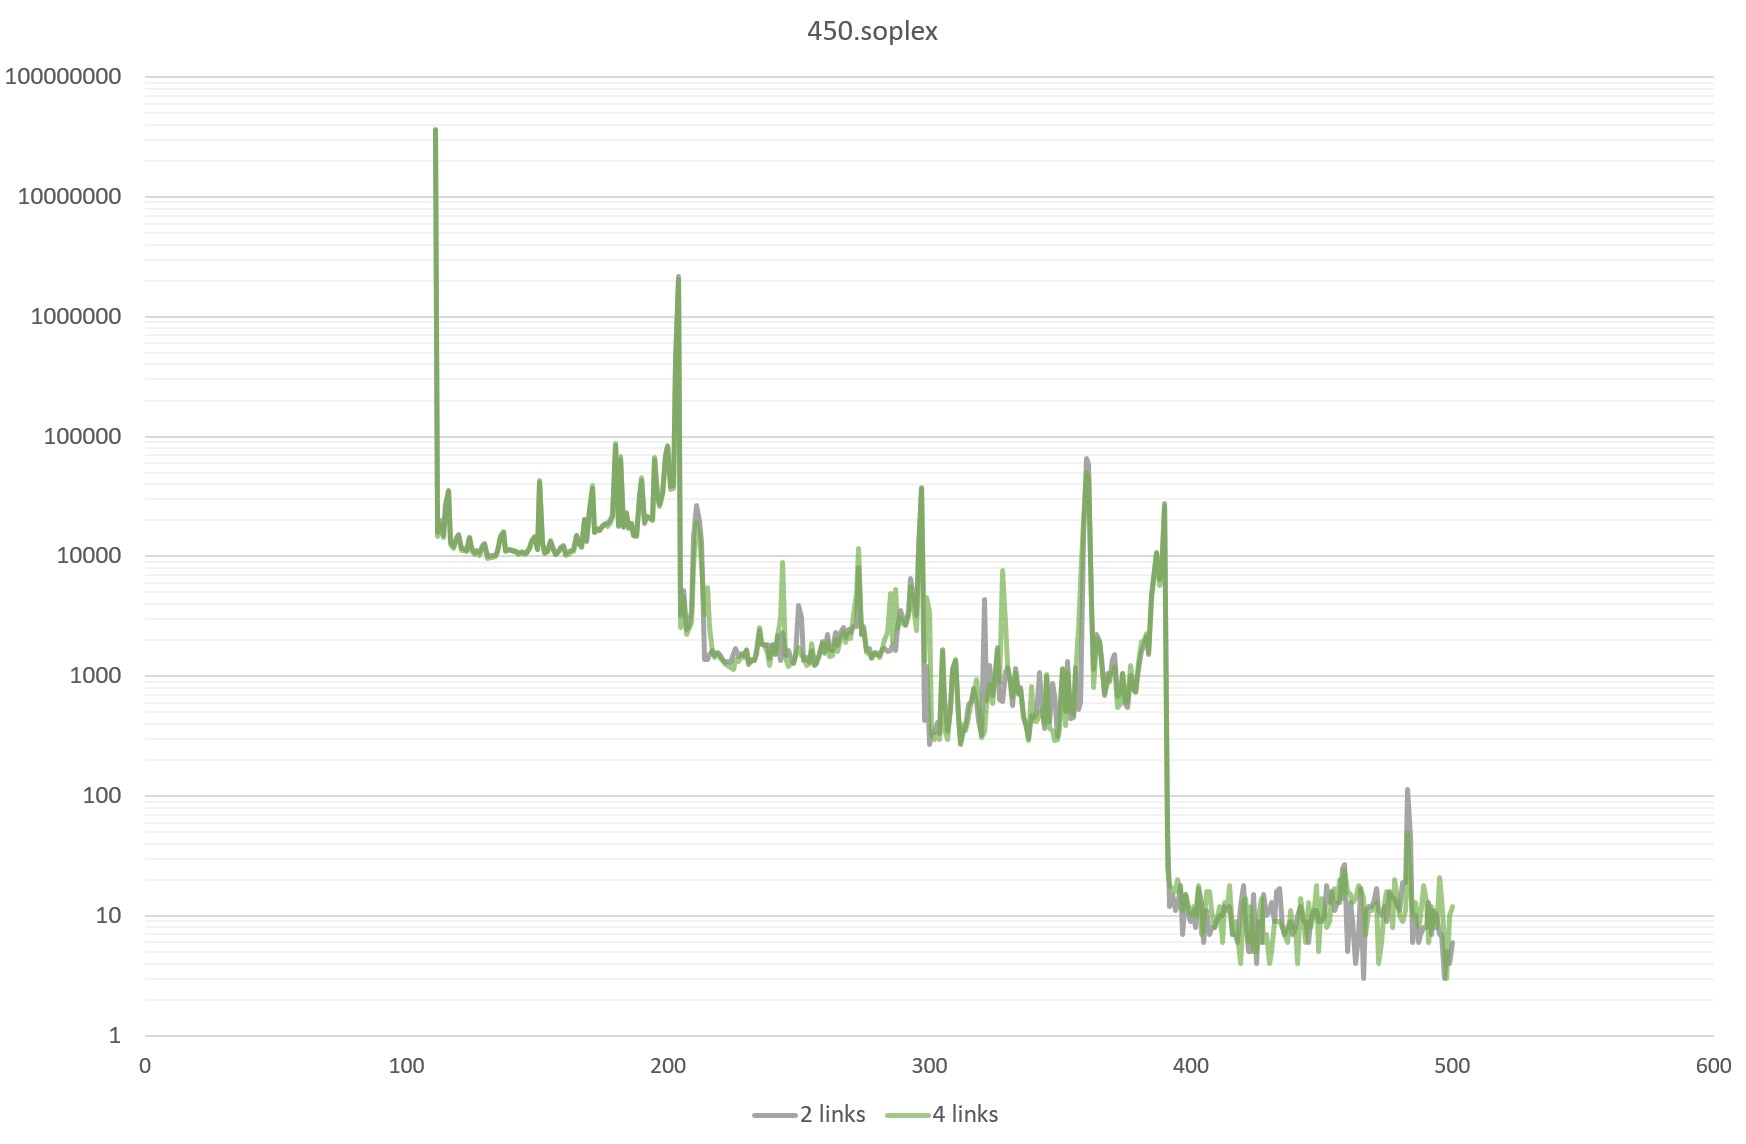
\includegraphics[width=1.0\linewidth]{figure/450-4_4-8.jpg}
    \caption{Nearly identical latency with two and four links when using three devices.}
    \label{Memory-access-450-4-dev-4-8-links}
\end{figure}

However, although the difference in average latency likely is very small, there is a performance gain, albeit small, as can be seen in figure \ref{Memory-access-450-exectime}. While the difference in execution time is small, it is not entirely too small to disregard. Furthermore, another interesting insight is that using one device with added links does \emph{not} increase performance -- it stays approximately the same. Soplex's algorithm could behave in such a way that the increase in latency for the otherwise fastest accesses using one device with more links counters the added bandwidth, while the overall higher \emph{average} latency for three devices is low enough for the application to be able to utilise BLP better. Memory accesses could be spread out sufficiently well to see some form of gain.
\bigskip

\begin{figure}[!ht]
    \centering
    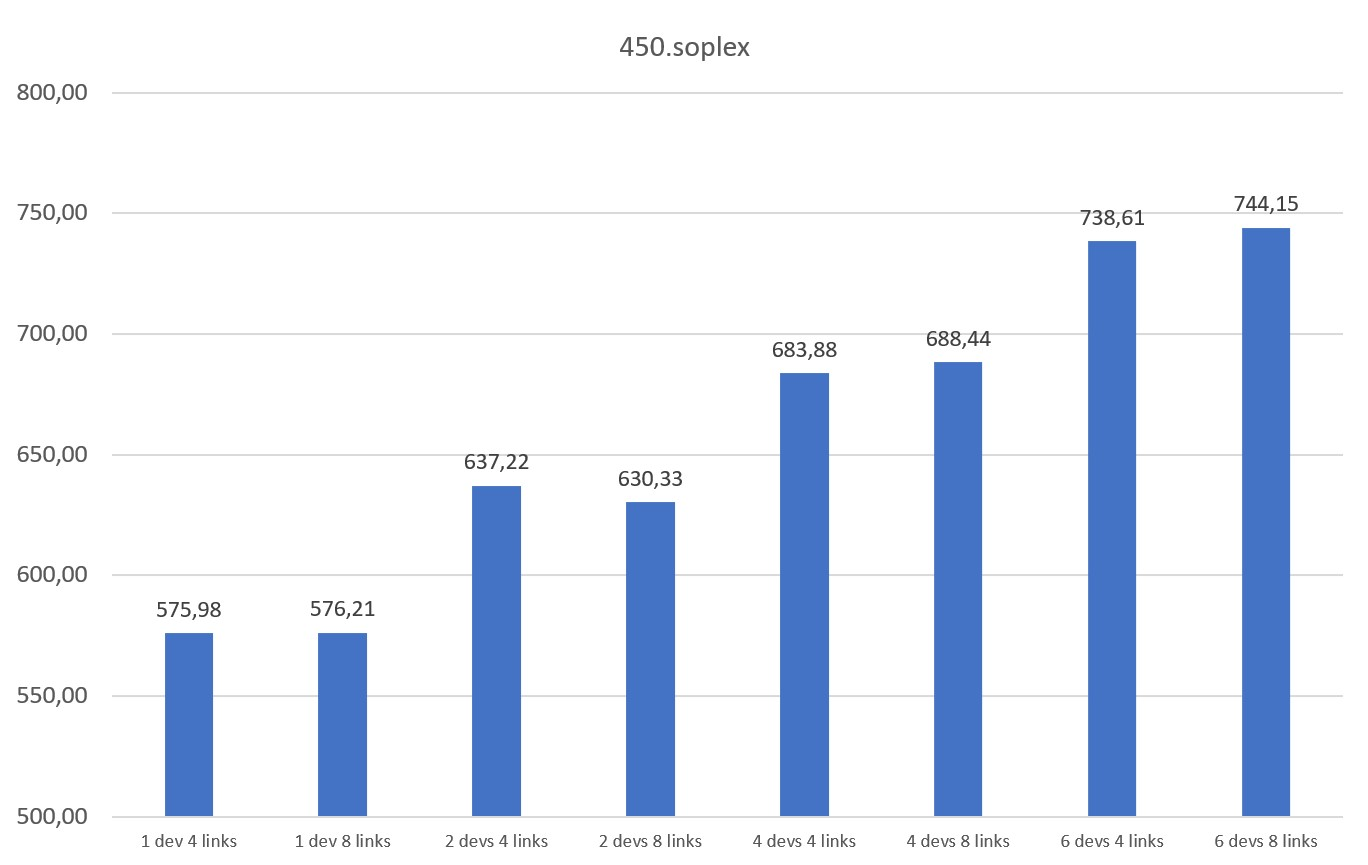
\includegraphics[width=1.0\linewidth]{figure/450-exectime.jpg}
    \caption{Execution time in ms for different configurations.}
    \label{Memory-access-450-exectime}
\end{figure}

This application's IPC variations over time does not seem to follow any discernable pattern, likely giving rise to few stream memory accesses \cite{song2018experiments}. Furthermore, this leads to about 88\% of all accesses being able to return in 93 ns and keeping the average latency low. Otherwise we see a familiar pattern in figure \ref{Memory-access-450-2-dev-4-8-links}, where additional spikes arise 9 ns behind the largest peaks when using four links and allocating data on the device next to the CPU. This also affects the average latency in this configuration, making it three ns slower compared to using only two links due to this phenomena. As seen before, however, this behaviour seems to be isolated to having more links available when allocating close to the host. 
\bigskip

\begin{figure}[!ht]
    \centering
    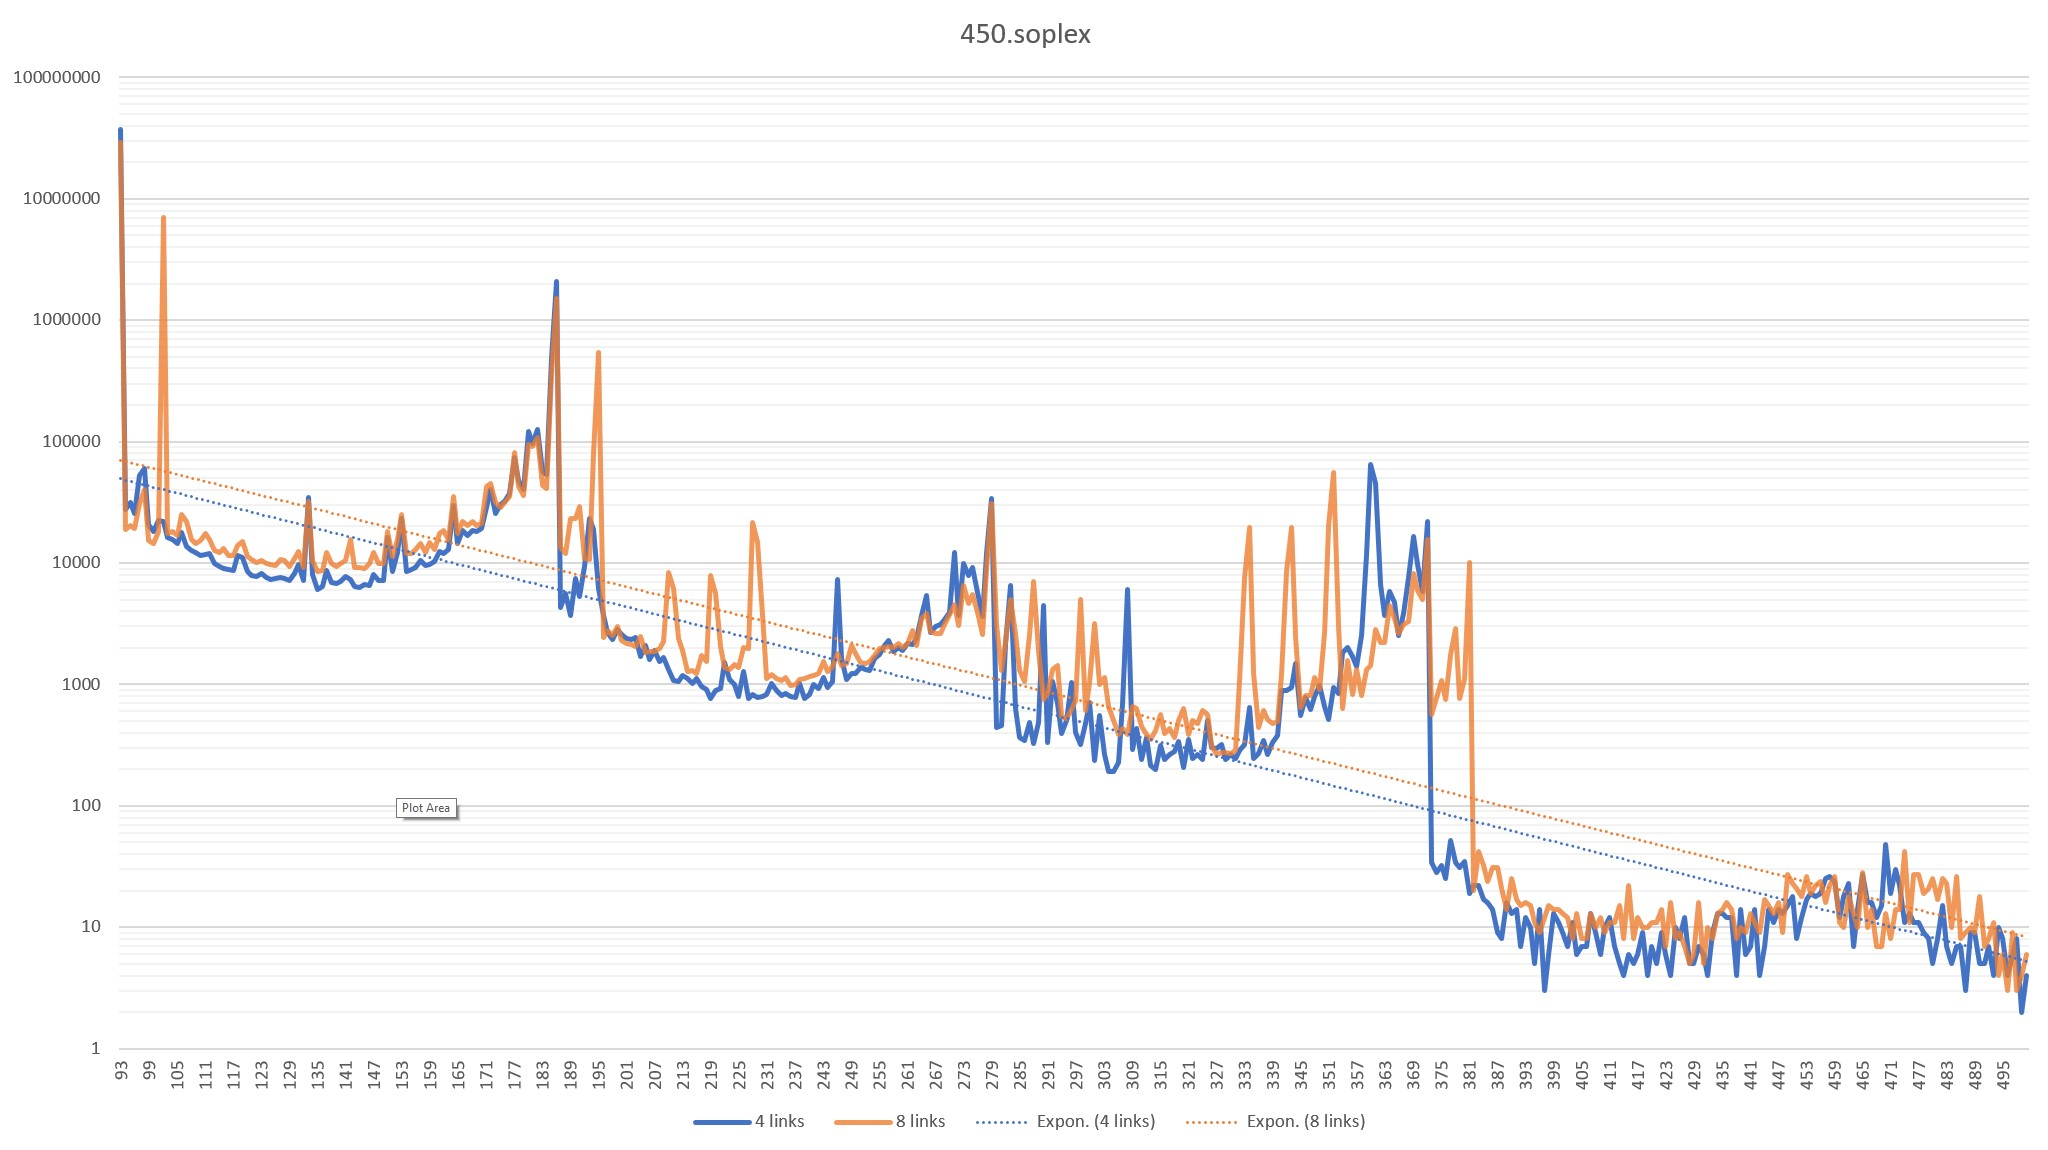
\includegraphics[width=1.0\linewidth]{figure/450-2_4-8.jpg}
    \caption{Using four links close to the processor creates additional spikes.}
    \label{Memory-access-450-2-dev-4-8-links}
\end{figure}

\section{LBM}
The access time pattern for 470.lbm resembles that of namd, where the main peak is at 186 ns. One major difference is the number of memory requests created by the application, which makes it possible to identify the repeating pattern even after a few hundred nanoseconds -- the graph in figure \ref{Memory-access-470} displays a distinct pattern where access latencies drop off very quickly after the last peak around 400 ns (note that the graph has been cut at 500 ns for compactness). Moreover, lbm almost exclusively uses stream memory accesses, more than 95\% of all accesses are done this way \cite{10.1145/3307650.3322229}. Additionally, most streams are very long, which would put a large strain on the HMC queues and could create patterns where the main peak comes in later than the optimal 93 ns \cite{8366939}. Furthermore, while lbm does issue a large amount of memory accesses, we infer from its IPC variations over time that streams are fetched and processed immediately \cite{song2018experiments}. This could be the reason why lbm does not have many requests waiting more than 4 * 93 ns, as opposed to mcf, despite its large total number of memory operations. If there were longer periods of time with sustained memory access, we believe there would be an increased amount of latencies after the current 400 ns break. 
\bigskip

\begin{figure}[!ht]
    \centering
    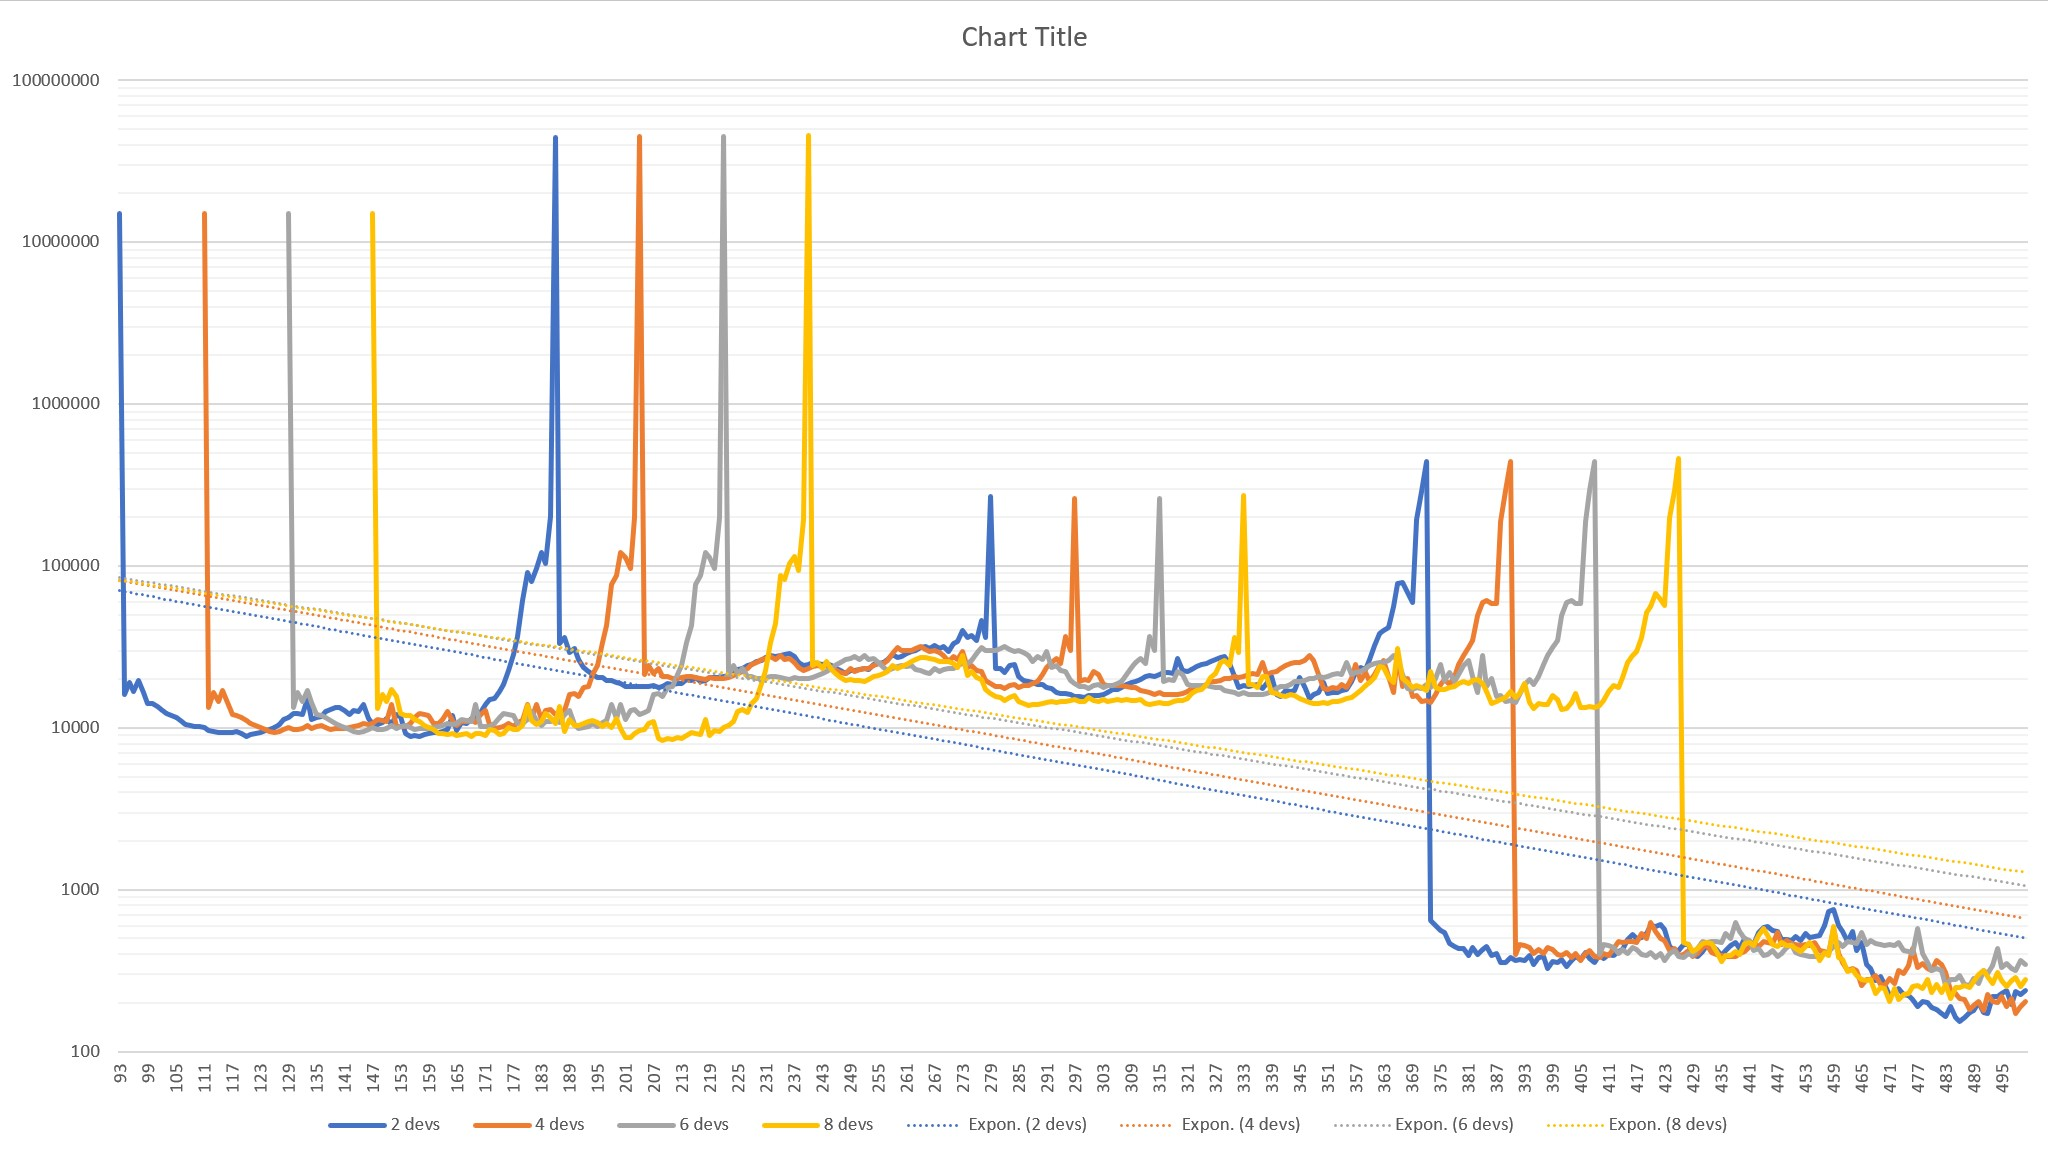
\includegraphics[width=1.0\linewidth]{figure/470-x_4.jpg}
    \caption{Comparing access time patterns between configurations.}
    \label{Memory-access-470}
\end{figure}

The same behaviour is seen when using two and four links close to the CPU, i.e. only having one device, is present when running lbm. Furthermore, there appears to be the same addition of latency when having to do internal routing in the first cube, where two ns of average latency is added, as seen in figure \ref{Memory-access-470-averages}. Lastly, it should be noted that running lbm using four links and seven devices took too long to complete and the session was terminated without any result available. However, based on the trends present among this and the other results, the outcome does not look very difficult to guess.
\bigskip

\begin{figure}[!ht]
    \centering
    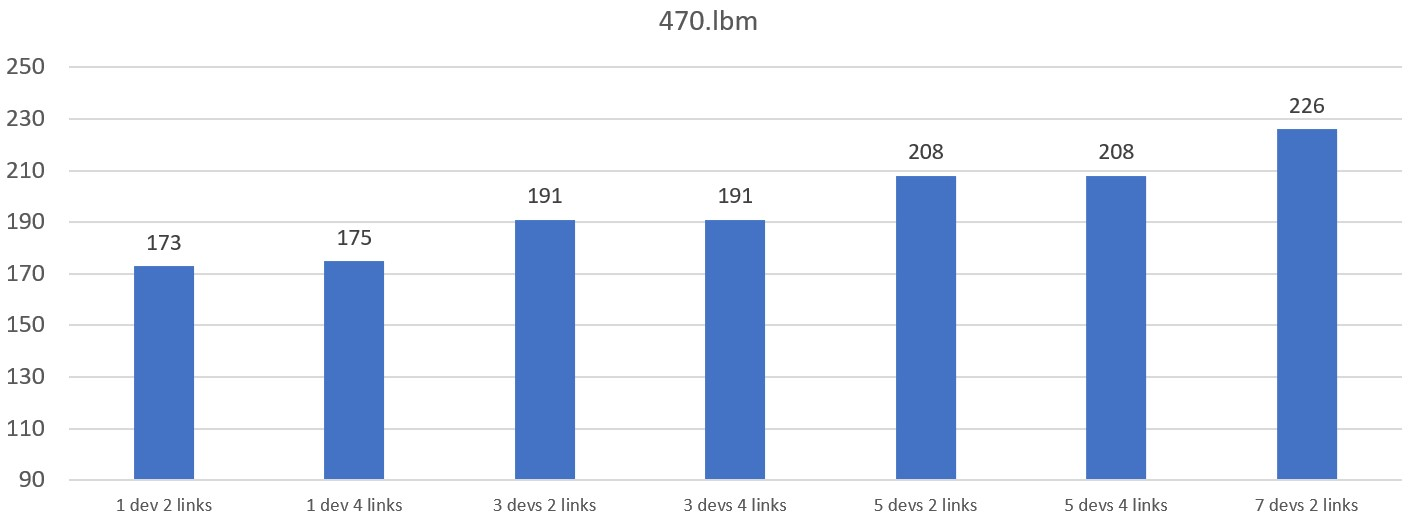
\includegraphics[width=1.0\linewidth]{figure/470-averages.jpg}
    \caption{Comparing average latency between configurations.}
    \label{Memory-access-470-averages}
\end{figure}

Figure \ref{Memory-access-470-exectime} shows that running lbm took between 1,1 and 1,5 seconds depending on configuration. Looking at running with three devices and adding two more links, we observe that there is a very small decrease in execution time. This difference is merely two ms, which in its context looks insignificant, but comparing to soplex's seven ms it gains some credibility. Soplex showed a very similar behaviour with respect to being able to utilise increased bandwidth even though the average latency increased from having data placed further away. However, given the differences in scale, this result could also be within the margin of error for simulations.
\begin{figure}[!ht]
    \centering
    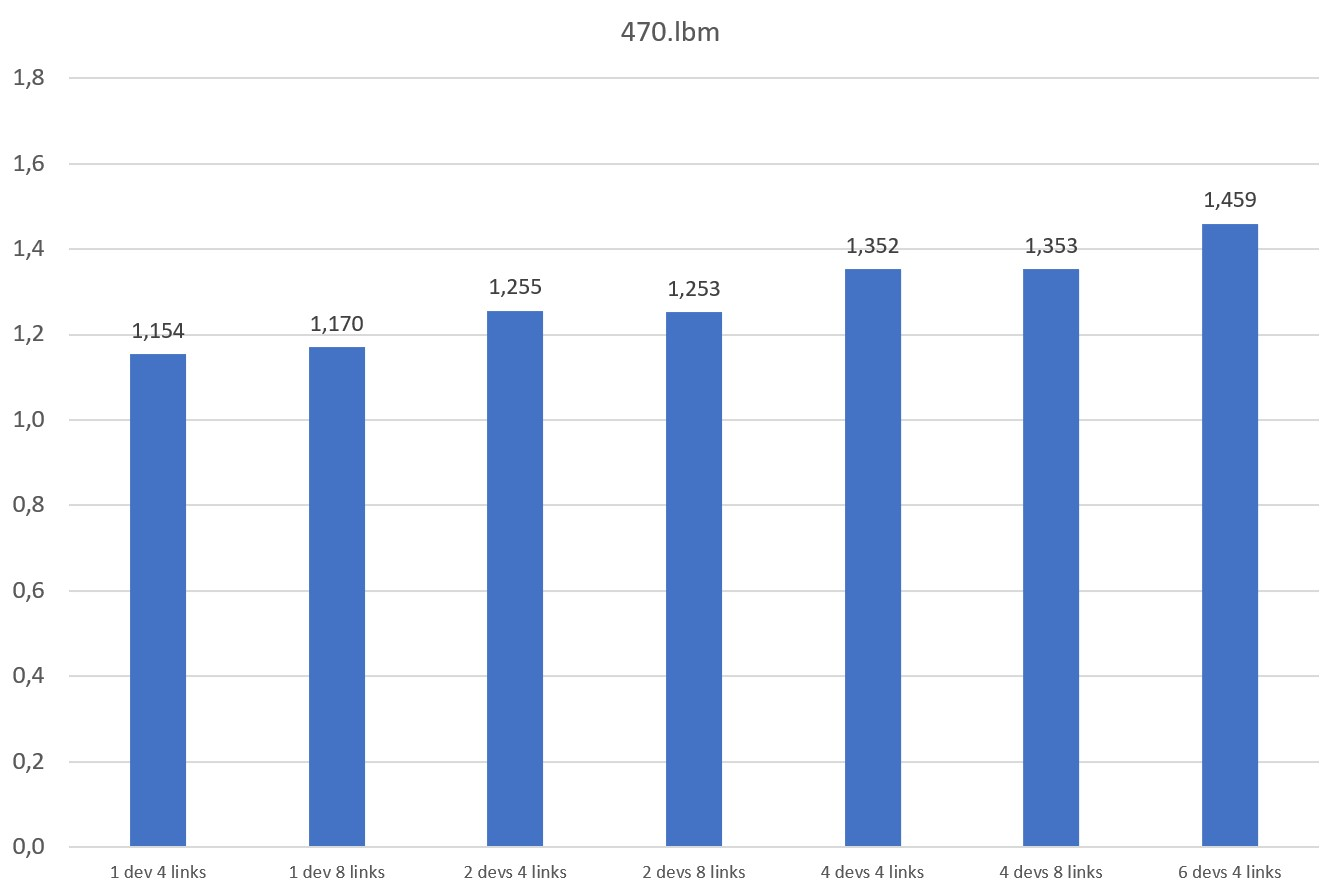
\includegraphics[width=1.0\linewidth]{figure/470-exectime.jpg}
    \caption{Execution time in seconds for different configurations.}
    \label{Memory-access-470-exectime}
\end{figure}

\section{OMNETPP}
Finally 471.omnetpp is run and similarly to soplex, a large portion, 89\%, of all requests are returned in 93 ns. While being a memory intensive application, omnetpp is highly parallel and in this case accesses many individual memory items at a time, and only about 5\% of memory accesses are streams \cite{10.1145/3307650.3322229}. Nevertheless, as can be seen in figure \ref{Memory-access-471}, there are enough accesses done simultaneously at times to cause congestion in the queues.
\bigskip

\begin{figure}[!ht]
    \centering
    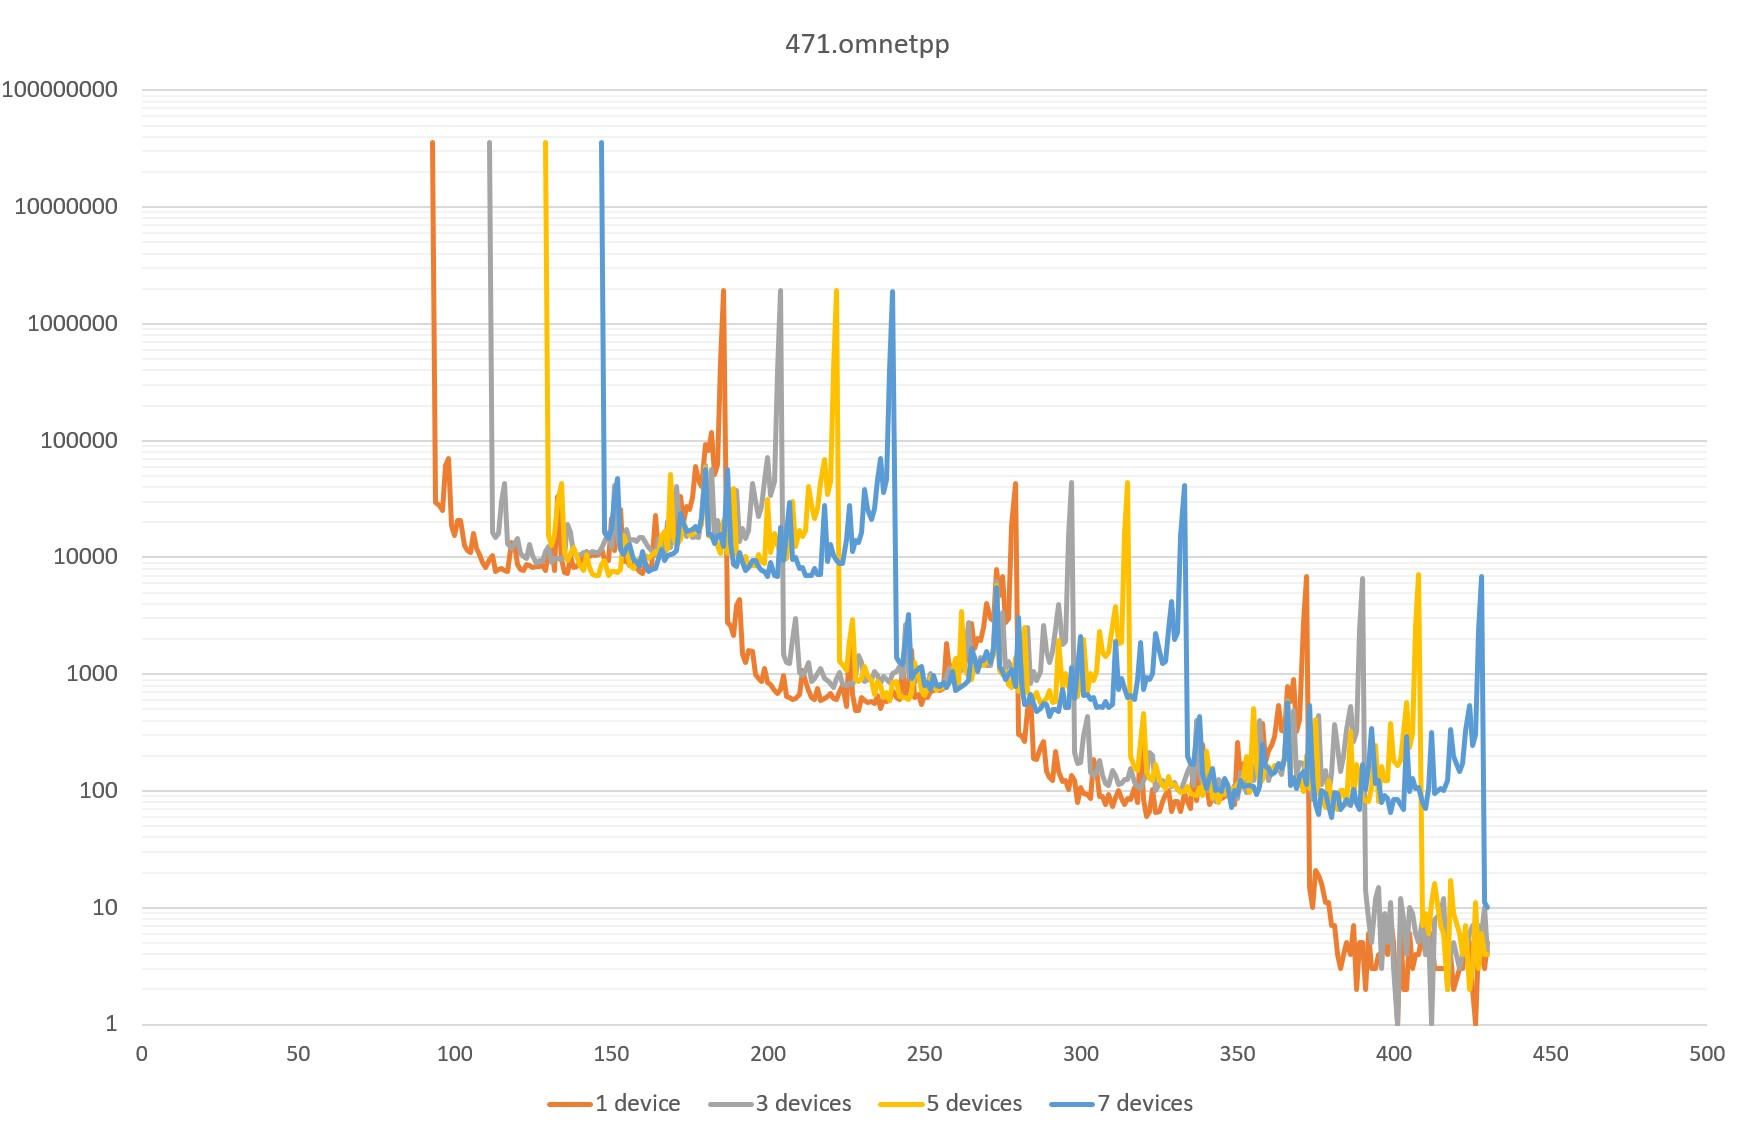
\includegraphics[width=1.0\linewidth]{figure/471-x_4.jpg}
    \caption{Comparing access time patterns between configurations.}
    \label{Memory-access-471}
\end{figure}

These accesses are done to different parts of memory where data was originally allocated, which should increase the amount of internal routing needing to be done. As can be seen in figure \ref{Memory-access-471-link-compare}, we have the familiar pattern of 9 ns delay for a portion of the first peak -- in this case almost 25\%. This added latency is, as seen previously, not present when using devices further away in the network. Additionally, average latency is increased by two ns when using four links, as seen in figure \ref{Memory-access-471-averages}, which seems comparatively low considering how many percent of requests are delayed.
\bigskip

\begin{figure}[!ht]
    \centering
    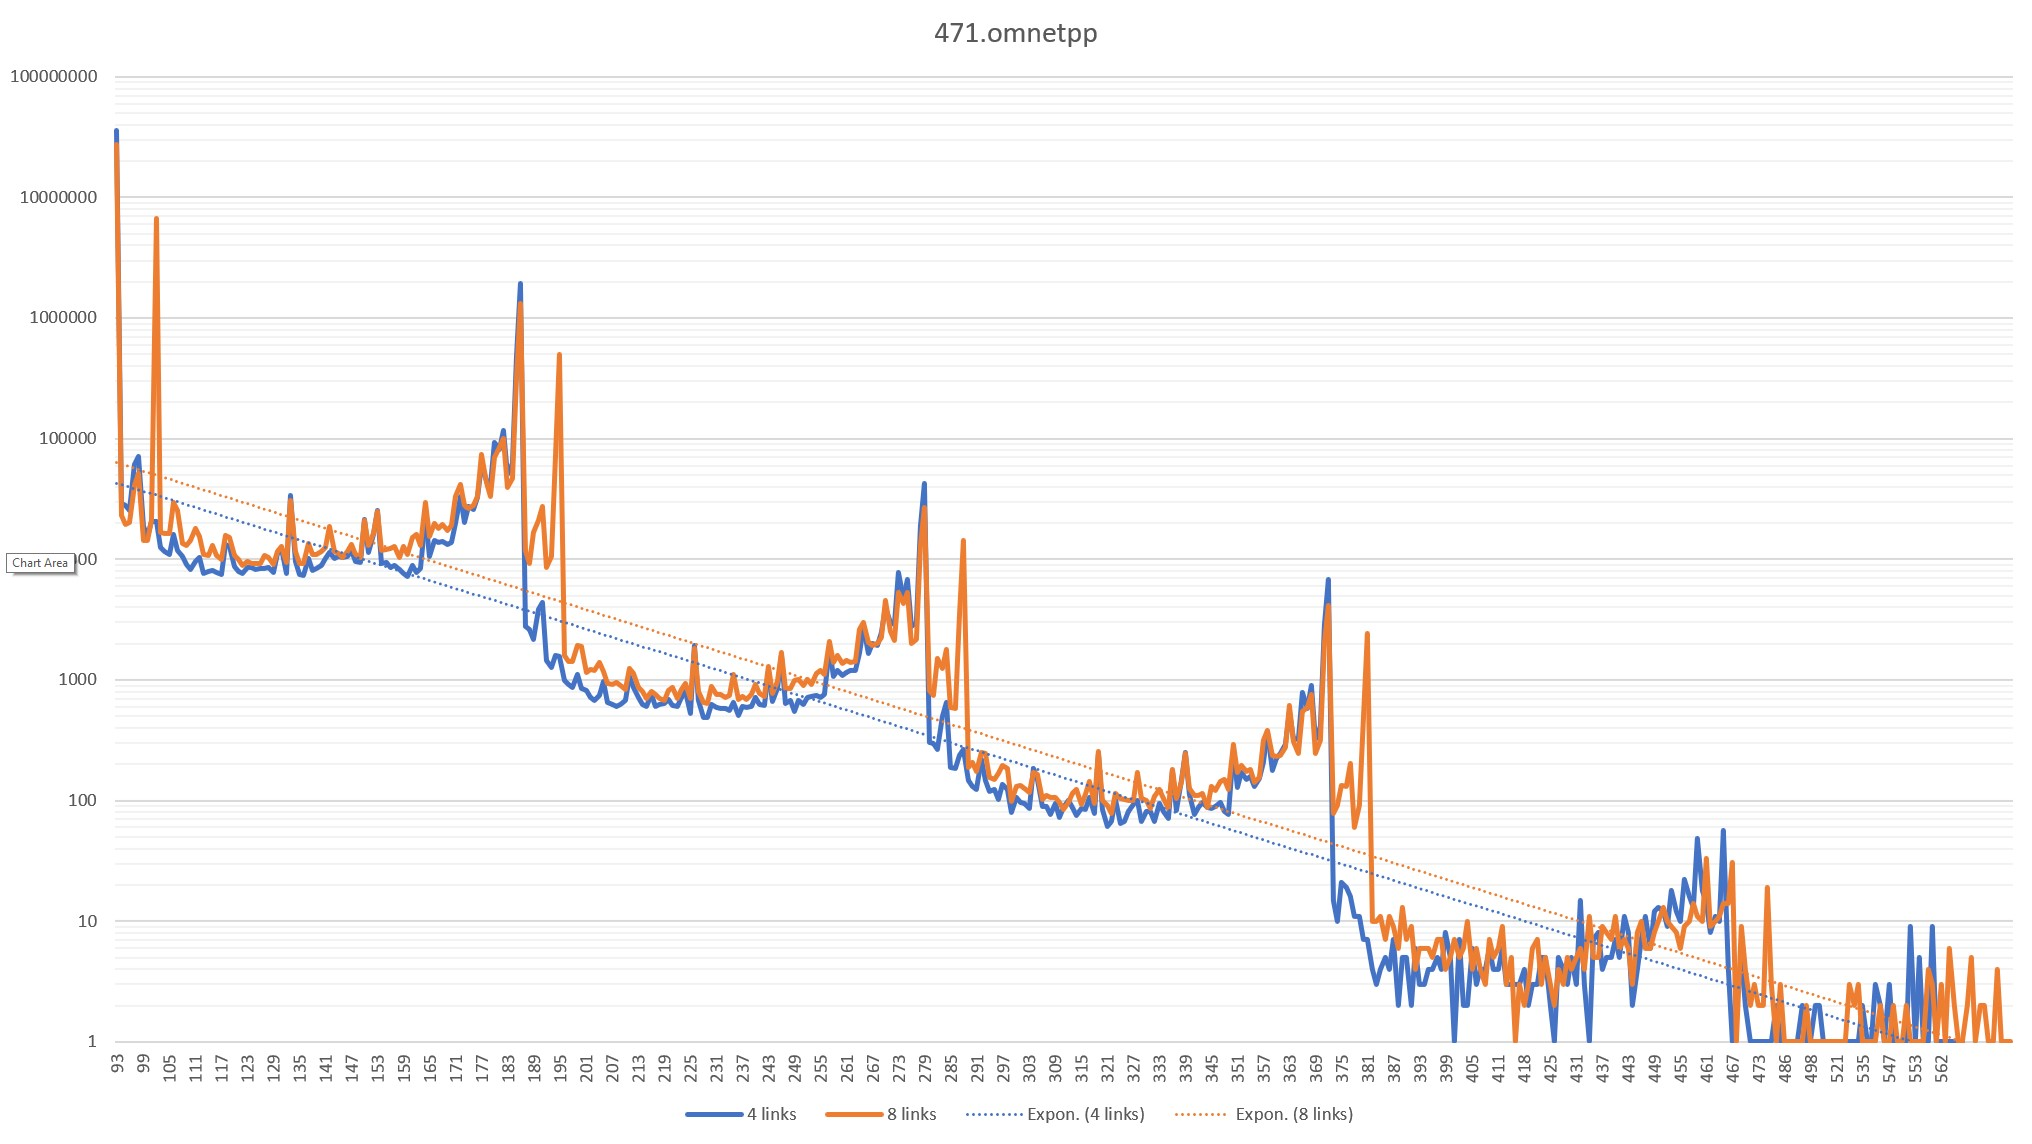
\includegraphics[width=1.0\linewidth]{figure/471-2_4-8.jpg}
    \caption{Using four links causes internal routing and delays some requests.}
    \label{Memory-access-471-link-compare}
\end{figure}

\begin{figure}[!ht]
    \centering
    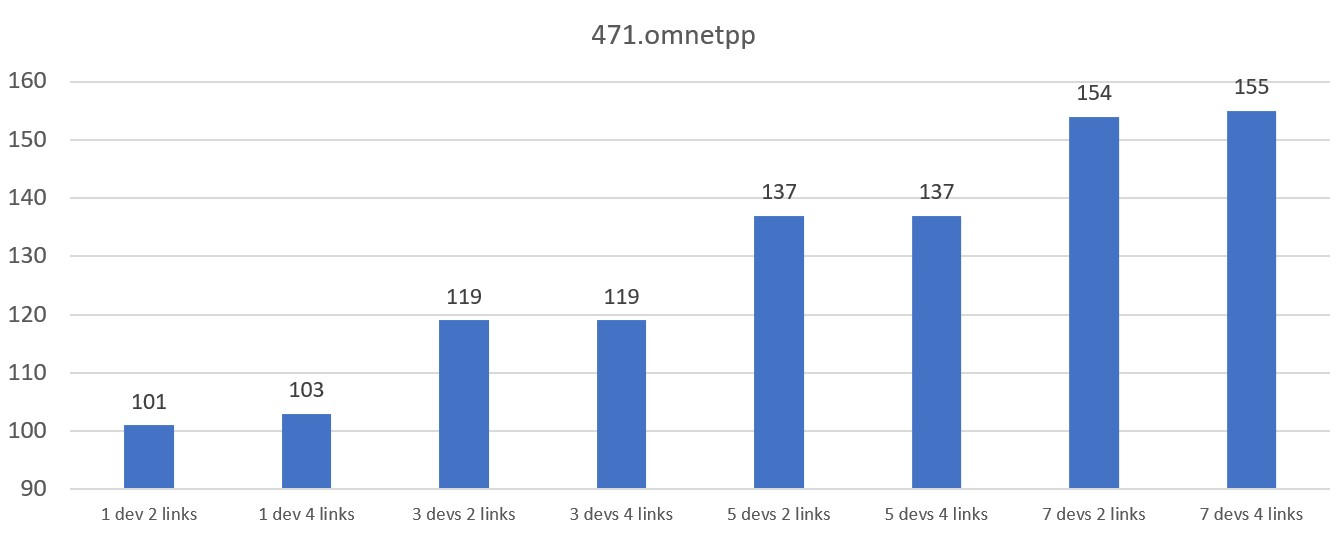
\includegraphics[width=1.0\linewidth]{figure/471-averages.jpg}
    \caption{Comparing average latency for different configurations.}
    \label{Memory-access-471-averages}
\end{figure}

With omnetpp we notice a performance gain when using one device with four active links, as seen in figure \ref{Memory-access-471-exectime}, despite experiencing a longer average access time. There is a trade-off to be made between latency and bandwidth, and in this case the need for high bandwidth outweighs the slightly increased latency. In addition, the low amount of stream memory access, while remaining mostly memory bound, as partially inferred from its IPC variations over time, could be interpreted as a good distribution of memory requests especially suitable for HMC's network model \cite{song2018experiments}. Furthermore, the notable reduction of 11 ms to the execution time means that omnetpp could utilise the added BLP well, but when the average latency grows further the application can no longer continue to supply new requests at a sufficient rate thus lowering effective bandwidth \cite{10.1145/3167132.3167249}. 

\begin{figure}[!ht]
    \centering
    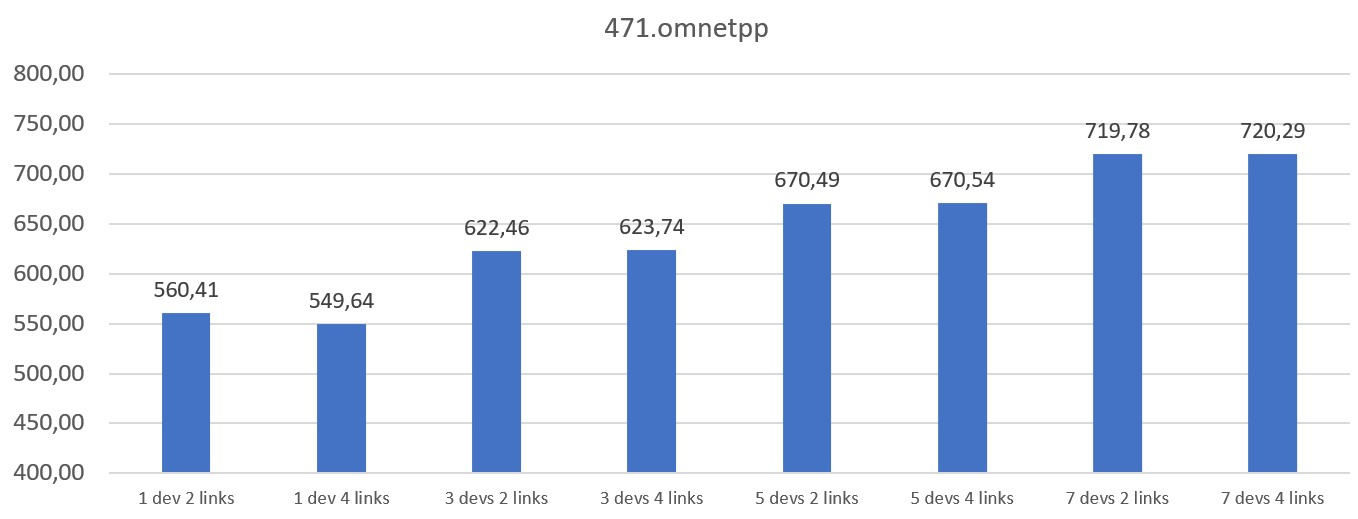
\includegraphics[width=1.0\linewidth]{figure/471-exectime.jpg}
    \caption{Execution time for different configurations.}
    \label{Memory-access-471-exectime}
\end{figure}

\section{Summary}
The Hybrid Memory Cube's use of a packet-based protocol means that it uses queues to process incoming and outgoing packets and these queues will fill up quickly if an application issues multiple memory requests in short succession \cite{8366939}. When applications' core use streamed memory accesses, a lot of requests will be sent in order to retrieve sequential data. This of course depends on the application and how its main algorithm operates, where some display this behaviour for most of its accesses and others have none \cite{10.1145/3307650.3322229}. Streamed memory access is an access behaviour which does not cache well and therefore will generate a lot of requests to main memory, which for HMC in turn means a lot of requests ending up in the queues in a short time frame. While the queues are filling up, i.e. not full, the memory's bandwidth is not fully utilised. The opposite is true as well, where full queues will enable the memory to work at full bandwidth, although at an increased latency. Furthermore, it is hard to determine what average latency an application will experience, where lbm for example exhibits a high average latency but quite a controlled variance due to its burst-like access pattern. While stream memory access generates many requests in a short time frame, there are likely other access patterns which could cause similar behaviour as well and in turn unwittingly cause significantly increased average latency.
\bigskip

Doubling the number of available links will increase possible bandwidth, but our tests show that more links also add internal routing which in turn adds routing latency. Depending on the application, this is either beneficial to or hampering performance, based on what its access patterns look like. With our setup we saw that when adding more links and using the HMC device closest to the CPU, around 20-25\% of accesses were delayed an additional 9 ns. This is likely due to requests ending up in the wrong quadrant and having to be re-routed to the correct one. Moreover, this behaviour is masked when using any other device at least two hops away. As such, there is no additional effect to latency due to allocating data far away, apart from the transfer time.
\bigskip

As expected, there appears to be little gain in allocating data on a far-away device as compared to having it nearby. As can be seen in figure \ref{All-apps-latency}, all applications experience a linear gain in execution time as latency increases. Moreover, adding links will increase bandwidth and for some applications show a slight improvement to execution time, but this limited to when data resides on nearby devices. While there is an expected trade-off between bandwidth and latency, the bandwidth gain does not appear to outweigh the degradation in latency when allocating further away than three hops in the network \cite{10.1145/3167132.3167249}. As such, our four link configurations performs largely equal to the ones with two links when running a single application.
\bigskip

\begin{figure}[!ht]
    \centering
    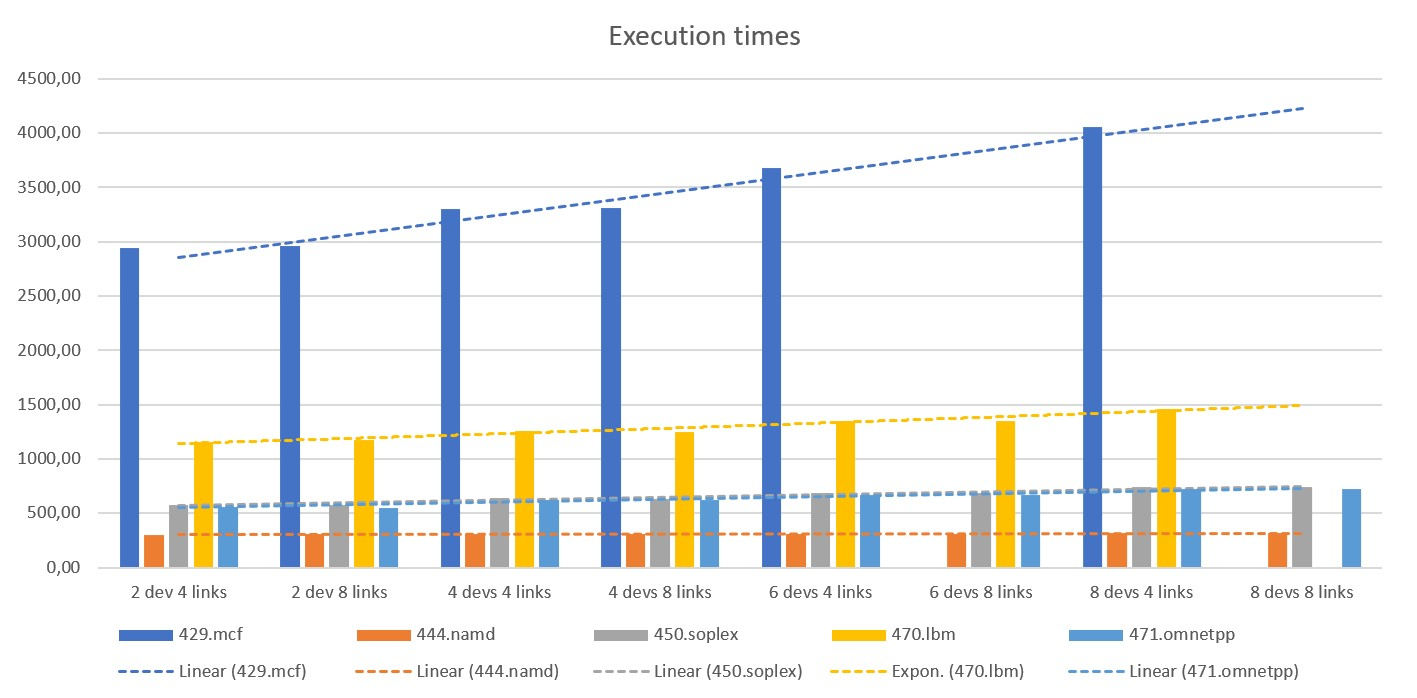
\includegraphics[width=1.0\linewidth]{figure/all-apps-exectime.jpg}
    \caption{Execution time for all applications and configurations.}
    \label{All-apps-latency}
\end{figure}

Lastly, the used applications react differently to the increase in average latency. Looking at figure \ref{All-apps-latency-trends} we can determine that the execution time for 429.mcf increases significantly more than the other, despite seeing the same latency increase during simulation. Likewise, 470.lbm, which is also a memory bound application, sees a higher increase than the rest. Observing the formula, in the form of {y=ax+b}, for each application, we assess that mcf is the most latency sensitive with {a=21}. 444.namd on the other hand presents very low sensitivity, with {a=0,2}.

\begin{figure}[!ht]
    \centering
    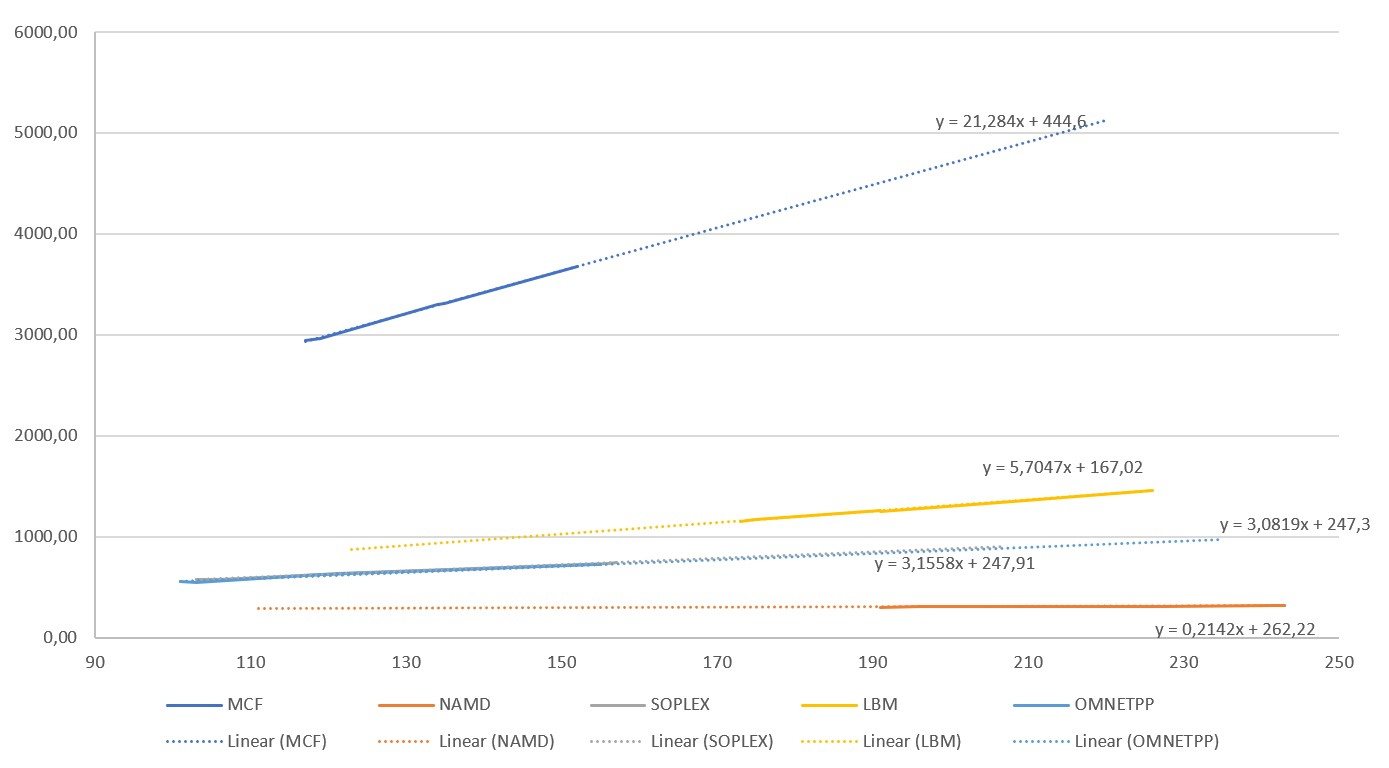
\includegraphics[width=1.0\linewidth]{figure/all-apps-latencies-trends.jpg}
    \caption{Applications' latency sensitivity, where a higher coefficient indicates higher degree of sensitivity}
    \label{All-apps-latency-trends}
\end{figure}